\documentclass[12pt,a4paper]{report}
\usepackage{graphicx}
\usepackage{amsmath}
\usepackage{booktabs}
\usepackage{xcolor}
\usepackage{hyperref}
\usepackage{float}
\usepackage{geometry}
\geometry{margin=1in}
\hypersetup{
    colorlinks=true,
    linkcolor=blue,
    urlcolor=blue,
    citecolor=blue
}

\begin{document}

%----------------------------------------
% Title Page
%----------------------------------------
\begin{titlepage}
  \centering
  {\scshape\LARGE Descriptive Statistical Analysis of Lionel Messi's Performance \par}
  \vspace{1.5cm}
  {\huge\bfseries Club and International Football (2010--2024) \par}
  \vspace{1.5cm}
  {\Large Course: MA2041 -- Probability and Statistics \par}
  \vspace{1cm}
  {\Large Instructor: Dr. Tanmay Sahoo \par}
  \vspace{1.5cm}
  {\Large Group Members \par}
  \vspace{0.8cm}

  \begin{center}
    \begin{tabular}{l}
      Member 1: Narahari Sai Rohan (142401026) \\
      Member 2: Parmar Manthan (142401027) \\
      Member 3: Piyush Dubey (142401028) \\
      Member 4: Prabhav Kumar (142401029) \\
      Member 5: Punit Yadav (142401030) \\
    \end{tabular}
  \end{center}



\tableofcontents
\newpage

%----------------------------------------
% 1. Introduction
%----------------------------------------
\chapter{Introduction}
Lionel Messi is widely regarded as one of the greatest footballers in history. His career has spanned over two decades, showcasing excellence both at the club level and on the international stage. This report provides a comprehensive descriptive statistical analysis of his performance from 2010 to 2024.

The goal of this analysis is to apply statistical measures such as mean, median, mode, variance, standard deviation, skewness, and kurtosis to quantify and interpret Messi's performance trends across years.

\section*{Objectives}
\begin{itemize}
    \item To analyze Messi's club and international performance from 2010--2024.
    \item To compute and interpret descriptive statistics for various performance metrics.
    \item To compare Club vs International trends using visual tools such as box plots and line charts.
\end{itemize}

%----------------------------------------
% 2. Data Collection and Sources
%----------------------------------------
\chapter{Data Collection and Sources}
The data used in this study was collected from reputable online sources:
\begin{itemize}
    \item \href{https://www.fotmob.com/players/30981/l-messi}{FotMob}
    \item \href{https://footystats.org/players/argentina/lionel-messi}{FootyStats}
    \item \href{https://fbref.com/en/players/d70ce98e/Lionel-Messi}{FBref}
\end{itemize}

These websites provide detailed match statistics including goals, assists, passes, shots, and advanced metrics such as expected goals (xG) and expected assists (xA). The dataset covers both Club and International matches.

%----------------------------------------
% 3. Variables and Their Definitions
%----------------------------------------
\chapter{Variables and Their Definitions}
The dataset contains the following key metrics:
\begin{itemize}
    \begin{itemize}
    \item \textbf{Matches Played:} The total number of official matches Messi participated in during a season, indicating his availability, consistency, and fitness.

    \item \textbf{Goals Scored:} The number of goals successfully scored by Messi, representing his direct contribution to the team's attacking output.

    \item \textbf{Assists:} The number of passes or actions delivered by Messi that directly resulted in a teammate scoring a goal, reflecting his playmaking ability.

    \item \textbf{Passes:} The total number of passes attempted during matches, showing Messi's involvement in possession and build-up play.

    \item \textbf{Successful Passes:} The total number of completed passes that reached the intended teammate, measuring accuracy and efficiency in ball distribution.

    \item \textbf{Pass Accuracy:} The percentage of attempted passes that were successfully completed, indicating technical precision and reliability in possession.

    \item \textbf{Dribbles:} The number of successful dribbles completed by Messi, demonstrating his ability to beat defenders, progress the ball, and create openings.

    \item \textbf{Shots on Target:} The number of shots that were directed towards the goal and required a save or resulted in a goal, reflecting shooting accuracy and threat level.

    \item \textbf{Minutes Played:} The total time Messi spent on the field during all matches in a season, signifying endurance, tactical importance, and match involvement.
\end{itemize}

\end{itemize}

%----------------------------------------
% 4. Methodology
%----------------------------------------
\chapter{Methodology}
Descriptive statistics were applied using Python (Pandas, NumPy, Matplotlib). The following measures were computed for each numeric variable:

\[
\text{Mean} = \frac{\sum x_i}{n}
\]
\[
\text{Variance} = \frac{\sum (x_i - \bar{x})^2}{n-1}
\]
\[
\text{Standard Deviation} = \sqrt{\text{Variance}}
\]
\[
\text{Skewness} = \frac{\sum (x_i - \bar{x})^3}{ns^3}
\]
\[
\text{Kurtosis} = \frac{\sum (x_i - \bar{x})^4}{ns^4}
\]

\section*{Tools Used}
\begin{itemize}
    \item Python 3.12+
    \item Pandas
    \item NumPy
    \item Matplotlib
    \item Excel for manual verification
\end{itemize}

%----------------------------------------
% 5. Data Analysis and Results
%----------------------------------------
\chapter{Data Analysis and Results}

\section{Descriptive Statistics Summary}
The following tables summarize Messi’s descriptive statistics for Club, International, and Combined performances.  

\subsection*{Table 1: Club Statistics}
\begin{table}[H]
\centering
\begin{table}[H]
\centering
\begin{tabular}{lcccccc}
\toprule
\textbf{Metric} & \textbf{Mean} & \textbf{Median} & \textbf{Variance} & \textbf{Std Dev} & \textbf{Skewness} & \textbf{Kurtosis} \\
\midrule
Matches & 47.133 & 49 & 73.695 & 8.585 & -0.140 & 2.321 \\
Goals & 42.333 & 41 & 271.810 & 16.487 & 0.694 & 2.642 \\
Assists & 18.733 & 18 & 34.781 & 5.898 & -0.013 & 2.607 \\
Passes & 1890.933 & 1883 & 64222.924 & 253.422 & -0.270 & 2.128 \\
Successful Passes & 1558.867 & 1529 & 317.171 & 17.809 & 0.085 & 1.964 \\
Pass Accuracy & 82.420 & 82.20 & 2.817 & 1.679 & 0.267 & 1.989 \\
Dribbles Success & 173.000 & 169 & 3841.714 & 61.982 & 0.582 & 2.395 \\
Shots on Target & 91.467 & 93 & 864.981 & 29.411 & -0.109 & 2.387 \\
Minutes Played & 3991.333 & 4067 & 602443.238 & 776.172 & -0.215 & 2.154 \\
\bottomrule
\end{tabular}
\caption{Descriptive Statistics for Messi’s Season-Wise Performance}
\end{table}

\caption{Descriptive statistics for Messi's Club performance}
\end{table}

\subsection*{Table 2: International Statistics}
\begin{table}[H]
\centering
\begin{tabular}{lcccccc}
\toprule
\textbf{Metric} & \textbf{Mean} & \textbf{Median} & \textbf{Variance} & \textbf{Std Dev} & \textbf{Skewness} & \textbf{Kurtosis} \\
\midrule
Matches & 9.800 & 10 & 11.886 & 3.448 & 0.203 & 1.920 \\
Goals & 6.533 & 6 & 16.552 & 4.068 & 1.025 & 4.302 \\
Assists & 3.267 & 3 & 6.495 & 2.549 & 0.442 & 2.510 \\
Passes & 394.333 & 395 & 1674.524 & 40.921 & -0.148 & 1.676 \\
Successful Passes & 318.667 & 315 & 1144.524 & 33.831 & -0.115 & 1.842 \\
Pass Accuracy & 80.760 & 80.70 & 1.598 & 1.264 & -0.489 & 2.318 \\
Dribbles & 29.800 & 28 & 122.600 & 11.072 & 0.587 & 2.446 \\
Shots on Target & 13.133 & 13 & 29.267 & 5.410 & 0.412 & 2.358 \\
Minutes Played & 835.400 & 810 & 93120.257 & 305.156 & 0.468 & 2.020 \\
\bottomrule
\end{tabular}
\caption{Descriptive Statistics for Messi’s International Performance}
\end{table}

    \begin{figure}[H]
      \centering
      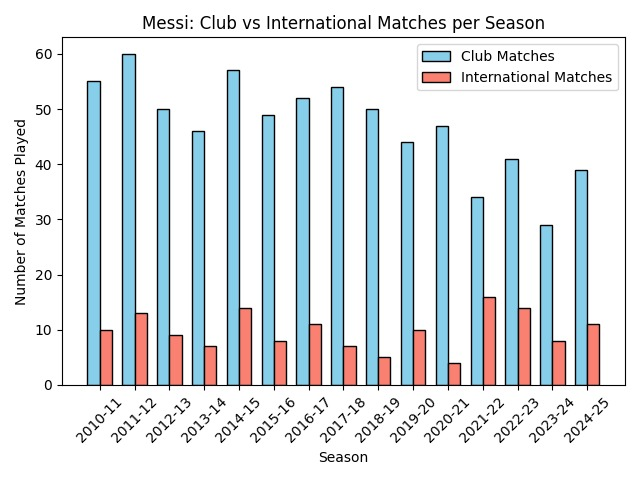
\includegraphics[width=0.9\linewidth]{WhatsApp Image 2025-11-13 at 15.43.20_dd64a0f2.jpg}
      \caption{}
      \label{fig:placeholder}
  \end{figure}
 This bar chart, titled "Messi: Club vs International Matches per Season," visualizes the sheer volume of Lionel Messi’s workload over a fifteen-year period from 2010-11 to 2024-25. The vertical axis represents the number of matches played, capping at 60, while the horizontal axis lists the seasons chronologically. The defining trend of the visual is the overwhelming dominance of club football (represented by light blue bars) compared to international duty (salmon-colored bars). In the early phase of the chart, particularly the 2011-12 season, Messi’s durability was at its absolute peak, with his club appearances hitting the maximum of 60 matches. For nearly a decade—from 2010 through 2019—he maintained a remarkably high baseline, rarely dipping below 50 club games per season, indicating his status as an indispensable starter who rarely rested.

However, a distinct shift becomes visible starting in the 2020-21 season. The height of the blue bars begins to recede significantly, dropping into the 30-40 match range for the 2021-22 and 2023-24 seasons. This trend likely reflects a combination of league changes, injury management, and natural aging. Meanwhile, the red international bars show a different pattern: they are less about volume and more about periodic variability. While typically staying between 5 and 10 matches, there are noticeable spikes in specific years—such as 2014-15 and 2021-22—which correspond to deep runs in major tournaments like the World Cup and Copa América. Interestingly, despite the reduction in his club workload in recent years, his availability for the national team has remained relatively stable.
  \begin{figure}[H]
      \centering
      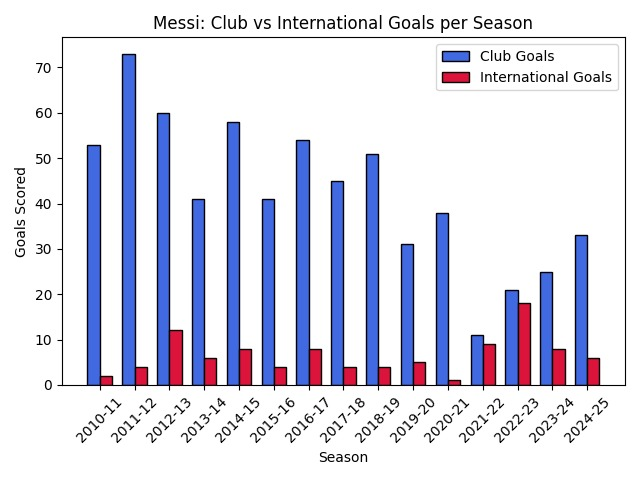
\includegraphics[width=0.9\linewidth]{WhatsApp Image 2025-11-13 at 15.47.29_97534884.jpg}
      \caption{}
      \label{fig:placeholder}
  \end{figure}
  This bar chart, "Messi: Club vs International Goals per Season," provides a striking visual record of Messi’s goal-scoring lethality. The scale here goes even higher than the matches chart, topping out at over 70, which is necessary to accommodate the chart’s most prominent feature: the colossal blue bar in the 2011-12 season. In that single year, Messi scored an unprecedented 73 club goals, a statistical outlier that towers over the rest of the graph. Following that historic peak, the chart displays a period of sustained excellence where the blue bars consistently hover between 40 and 60 goals for nearly eight consecutive seasons. This visual plateau demonstrates a decade-long era where scoring nearly a goal per game was his standard output.

The narrative of the graph changes drastically around the 2020-21 season. There is a sharp decline in club production, hitting a career-low trough in 2021-22 where the blue bar drops to roughly 11 goals—a stark contrast to his earlier heights. However, the red international bars tell a contrasting success story in the later years. For most of his career, international goals (red) were a small fraction of his total output, often barely visible on the scale. But in the 2022-23 season, the red bar surges dramatically to nearly 20 goals. This anomaly clearly visualizes his "World Cup" year, where his national team output essentially doubled his average, effectively compensating for the dip in his club statistics during that same period.
  \begin{figure}[H]
      \centering
      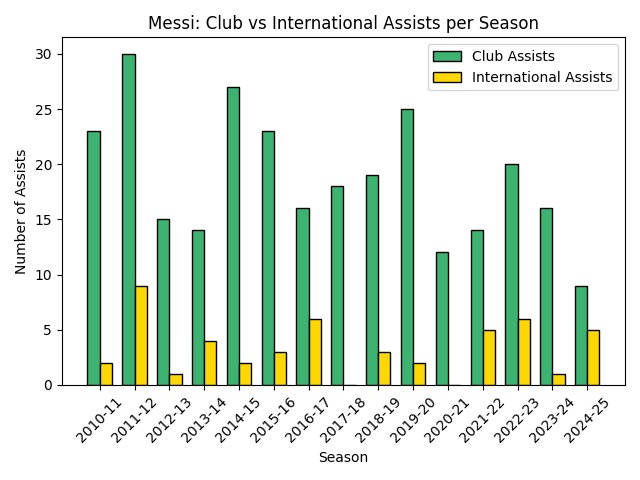
\includegraphics[width=0.9\linewidth]{WhatsApp Image 2025-11-13 at 15.51.08_6dbf7610.jpg}
      \caption{}
      \label{fig:placeholder}
  \end{figure}
  This bar chart, "Messi: Club vs International Assists per Season," highlights the creative side of Messi's game, tracking playmaking rather than finishing. The vertical axis here is scaled to 30, reflecting that assists are a rarer statistic than goals or passes. Unlike the "Matches" or "Goals" charts which show a relatively smooth decline over time, the green club assist bars here are much more volatile, showing three distinct peaks. The first peak aligns with his scoring prime in 2011-12 (reaching 30 assists), the second appears in 2014-15 (around 27 assists), and a third significant spike occurs in 2019-20 (25 assists). This third peak is particularly interesting because it happens much later in his career, suggesting that as his physical speed declined, he compensated by leaning more heavily into a creative role.

The yellow international assist bars are generally minimal throughout the timeline, often registering under 5 assists per season. However, the 2022-23 season again stands out as a late-career highlight. Just like with his goal scoring, there is a noticeable rise in both club and international assists during this specific season, with club assists rebounding to 20. The graph tapers off in the most recent 2023-24 and 2024-25 seasons, where both club and international numbers have dropped to their lowest combined levels on the chart, indicating a winding down of his prolific playmaking output.
  \begin{figure}[H]
      \centering
      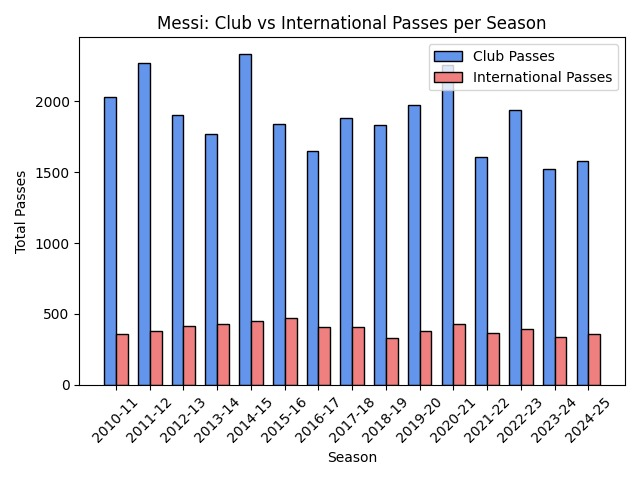
\includegraphics[width=0.9\linewidth]{WhatsApp Image 2025-11-13 at 15.54.08_35c9a609.jpg}
      \caption{}
      \label{fig:placeholder}
  \end{figure}
This bar chart, titled "Messi: Club vs International Passes per Season," offers a detailed quantitative breakdown of Lionel Messi’s involvement in play buildup across fifteen seasons, from 2010-11 to 2024-25. The vertical axis tracks the total volume of passes, scaling up to 2,500, while the horizontal axis organizes the data chronologically. The visual is dominated by the blue bars representing Club Passes, which consistently overshadow the red International bars, illustrating that the vast majority of his playmaking volume occurs at the club level. For most of the decade spanning 2010 to 2020, his club figures are staggering, frequently surpassing 1,800 passes per season and demonstrating his centrality to his team's possession-based style of play.

A closer examination of the club data reveals specific peaks and trends that likely correlate with tactical shifts. The highest volume of passes occurred in the 2014-15 season, where he surpassed 2,300 passes, with the 2011-12 season showing similarly high numbers. There is also a notable resurgence in passing volume in the 2020-21 season, where he once again broke the 2,000-pass barrier. However, the most recent three seasons (2022-23 through 2024-25) show a stabilized decrease, settling into a range of approximately 1,500 to 1,600 passes, which is lower than his historical average but still indicative of high involvement.

In stark contrast to the fluctuations seen in his club statistics, the red bars representing International Passes exhibit remarkable consistency. Unlike his goal or assist charts which show sharp spikes during tournament years, his passing metrics for the national team remain steady, almost exclusively hovering between 300 and 450 passes per season. This stability suggests that regardless of his fluctuating goal-scoring form or club environment, his fundamental role as a connector and distributor for Argentina has remained constant for over a decade. Even as his club output has trended slightly downward in recent years, his international passing volume has shown very little variance.
  \begin{figure}[H]
      \centering
      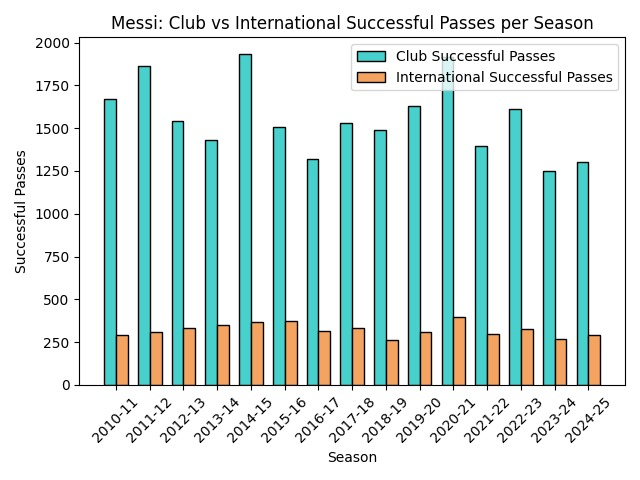
\includegraphics[width=0.9\linewidth]{WhatsApp Image 2025-11-13 at 15.56.39_56f3a78b.jpg}
      \caption{}
      \label{fig:placeholder}
  \end{figure}
This grouped bar chart, titled "Messi: Club vs International Successful Passes per Season," refines the data from the previous graph by focusing specifically on completed passes, serving as a proxy for his efficiency and retention of possession. The vertical axis scales up to 2,000, and the data spans from 2010-11 to 2024-25. The teal bars (Club Successful Passes) illustrate that his peak efficiency mirrors his peak volume; the 2014-15 season stands out as the highest point, where he completed nearly 2,000 passes. A second significant peak occurs in the 2020-21 season, again challenging the 2,000 mark, which underscores that even in his later years at Barcelona, he remained the primary hub of the team's circulation.

In contrast to the fluctuations in his club numbers—which show occasional dips in 2013-14 and 2015-16, and a clearer downward trend settling around 1,250 successful passes in the most recent seasons (2023-24 and 2024-25)—his international metrics display incredible stability. The orange bars (International Successful Passes) form a nearly flat line across the entire fifteen-year period, consistently hovering between 250 and 400 successful passes per season. This suggests that while his role at the club level evolved or his volume decreased with age and league changes, his tactical function for Argentina as a reliable link-up player has remained virtually unchanged for a decade and a half.
  \begin{figure}[H]
      \centering
      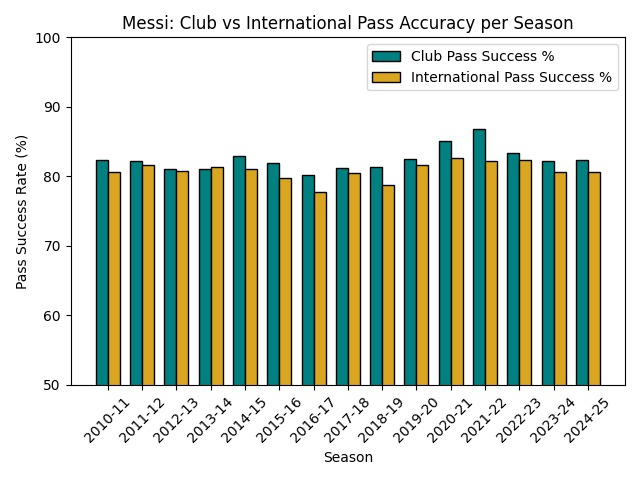
\includegraphics[width=0.9\linewidth]{WhatsApp Image 2025-11-13 at 16.08.29_529e1b3b.jpg}
      \caption{}
      \label{fig:placeholder}
  \end{figure}
  This grouped bar chart, titled "Messi: Club vs International Pass Accuracy per Season," shifts the focus from volume to precision, tracking the percentage of passes completed from 2010-11 to 2024-25. The vertical axis represents the Pass Success Rate, starting at 50 to better highlight marginal differences, while the teal (Club) and golden (International) bars show the data side-by-side. The most striking characteristic of this graph is its incredible stability; unlike the "Goals" or "Assists" charts which featured dramatic peaks and valleys, this visual forms an almost flat plateau. For over 15 years, Messi’s passing accuracy has consistently hovered between 80 and 87, regardless of the team he played for or the volume of passes he attempted.

A closer look at the teal club bars reveals a subtle but interesting trend: his highest efficiency actually occurred later in his career. While his physical volume (matches and goals) peaked in 2011-12, his technical precision peaked in the 2020-21 and 2021-22 seasons, where his club pass success rate climbed to its highest point on the chart, reaching approximately 87. This suggests that as he aged and his role shifted deeper into midfield, he became even more careful and precise with the ball. The golden international bars trail the club statistics slightly in most seasons but remain highly consistent, rarely dipping below 78 (with a minor dip in 2016-17). This consistency confirms that while his goal-scoring output for Argentina fluctuated, his reliability in possession was never in question.
  \begin{figure}[H]
      \centering
      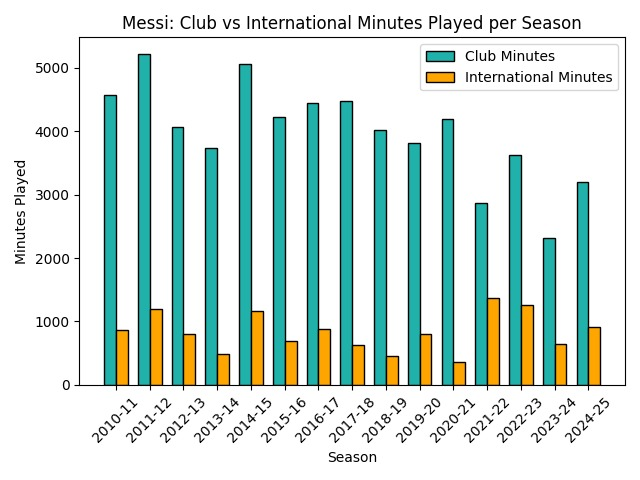
\includegraphics[width=0.9\linewidth]{WhatsApp Image 2025-11-13 at 16.10.49_a4d1cce5.jpg}
      \caption{}
      \label{fig:placeholder}
  \end{figure}
  This grouped bar chart, titled "Messi: Club vs International Minutes Played per Season," provides arguably the most accurate representation of Lionel Messi’s physical workload and durability over the last fifteen years. The vertical axis measures the total time spent on the pitch, scaling up to over 5,000 minutes, while the horizontal axis tracks the timeline from 2010-11 to 2024-25. The teal bars (Club Minutes) reveal the sheer magnitude of his endurance during his prime; specifically, in the 2011-12 and 2014-15 seasons, he surpassed the 5,000-minute mark. To put this into perspective, 5,000 minutes is roughly equivalent to playing 55 full 90-minute matches without being substituted, highlighting that for much of the last decade, he was virtually ever-present for his club.

The trend lines in this chart offer a clear narrative of his career stages. From 2010 through 2021, the club minutes remain incredibly high, rarely dipping below 4,000. However, a visible shift occurs starting in the 2021-22 season, where his club workload drops significantly to below 3,000 minutes, and hits a low point in 2023-24 (roughly 2,300 minutes). This decline likely reflects a transition to a league with fewer games or a conscious effort to manage his fitness. Conversely, the orange international bars show distinct spikes that align with major tournament cycles. Notably, the 2021-22 season shows one of his highest totals for international minutes (over 1,200), demonstrating that even as he scaled back his club activity, his commitment and availability for the national team during their critical winning era remained at its peak.
    \begin{figure}[H]
      \centering
      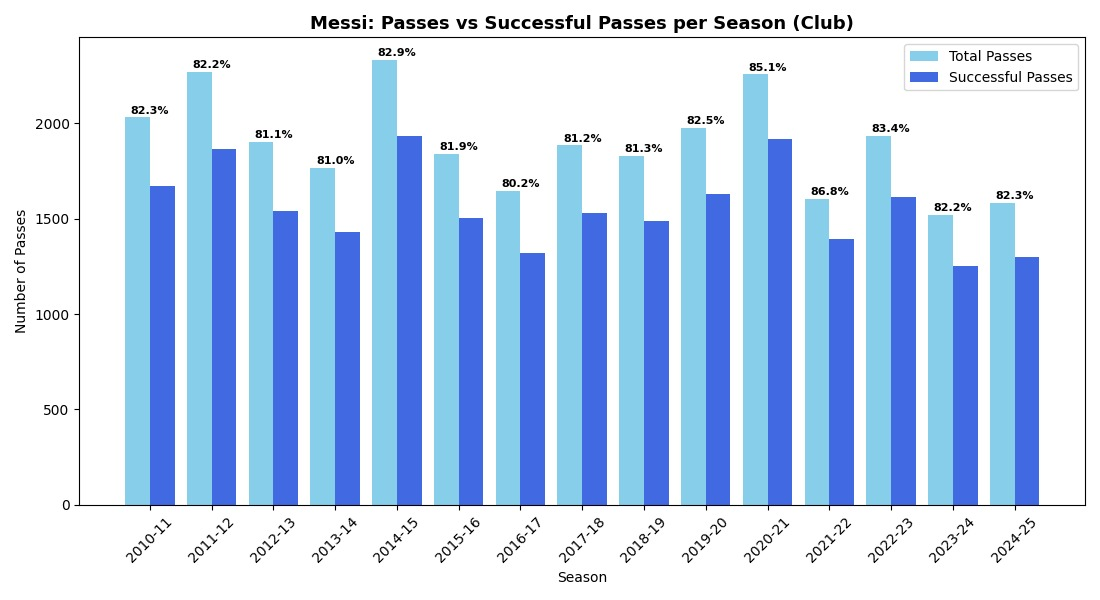
\includegraphics[width=0.9\linewidth]{WhatsApp Image 2025-11-13 at 16.29.36_cfd06a20.jpg}
      \caption{}
      \label{fig:placeholder}
  \end{figure}
  This specific chart, titled "Messi: Passes vs Successful Passes per Season (Club)," offers a granular look at Messi's passing efficiency strictly at the club level, removing international data to focus on his day-to-day league performance. The visual pairs "Total Passes" (light blue) with "Successful Passes" (dark blue) for each season from 2010-11 to 2024-25, but its most valuable feature is the data labels sitting atop the bars, which explicitly state his pass completion percentage for each year. While the volume trends align with previous charts—showing massive peaks in 2011-12 and 2014-15 where total passes exceeded 2,300—the percentages reveal a fascinating evolution in his playing style.

For the first decade of the chart (2010 to 2019), his passing accuracy was remarkably consistent, hovering steadily between 80.2 and 82.9. This consistency occurred even as his role fluctuated between a false nine and a right winger. However, a distinct shift in precision occurs in the 2020-21 and 2021-22 seasons. Even as his total pass volume began to decrease slightly from his absolute peak, his efficiency spiked, reaching a career-high 86.8 in 2021-22 and 85.1 in 2020-21. This statistical jump strongly suggests a change in tactical role during his final years at Barcelona and first year at PSG, where he likely dropped deeper into midfield to dictate play with safer, more calculated distribution rather than attempting as many high-risk final-third passes.
  \begin{figure}[H]
      \centering
      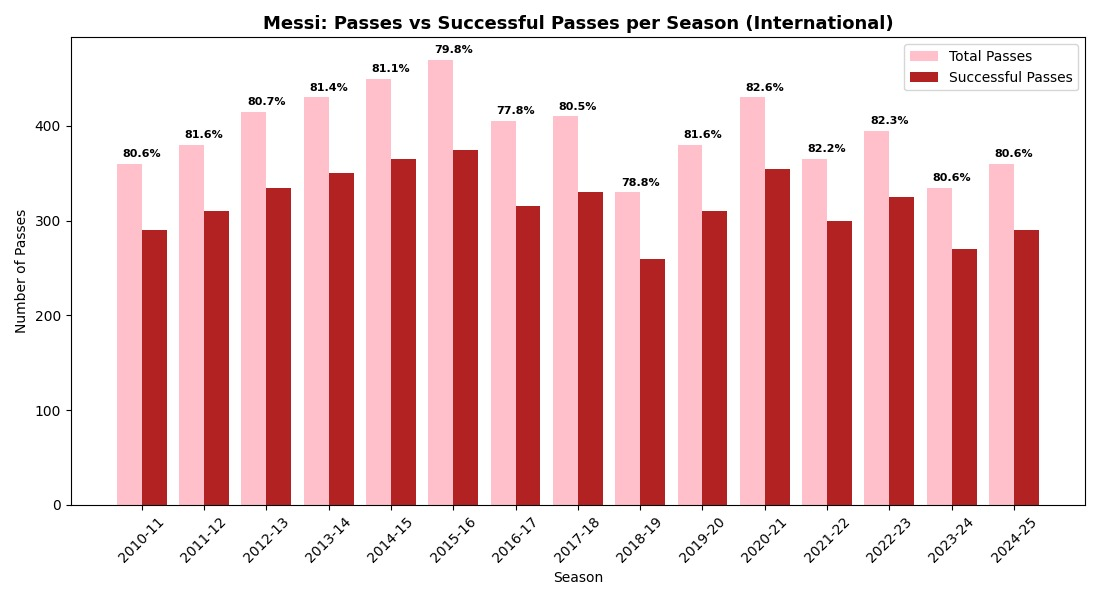
\includegraphics[width=0.9\linewidth]{WhatsApp Image 2025-11-13 at 16.29.44_76f24d95.jpg}
      \caption{}
      \label{fig:placeholder}
  \end{figure}
  This chart, titled "Messi: Passes vs Successful Passes per Season (International)," serves as the direct counterpart to the previous club-focused graph, isolating his passing performance solely for the Argentina national team. The visual pairs "Total Passes" (pink) with "Successful Passes" (dark red) across the same 2010-2025 timeline, using data labels to explicitly display the pass completion percentage for each season. The most defining characteristic of this dataset is its extraordinary stability. Unlike his club metrics, which showed clear evolutionary phases in accuracy, his international passing reliability has remained locked in a incredibly tight window—hovering between 78% and 82% for virtually his entire career.

While the volume of passes fluctuates significantly depending on the international calendar—peaking in 2014-15 (over 450 passes) and 2020-21 (around 430 passes), likely due to major tournaments like the Copa América and World Cup qualifiers—his efficiency rarely wavers. The highest recorded accuracy on the chart appears in the 2020-21 season at 82.6, coinciding with the period leading up to his first major international trophy. Even in the most recent seasons (2022-23 through 2024-25), after achieving World Cup glory, his pass completion rate remains steadfast above 80, confirming that his ability to retain possession and distribute the ball effectively for his country has been a constant, unwavering baseline regardless of the team's broader performance.
      \begin{figure}[H]
      \centering
      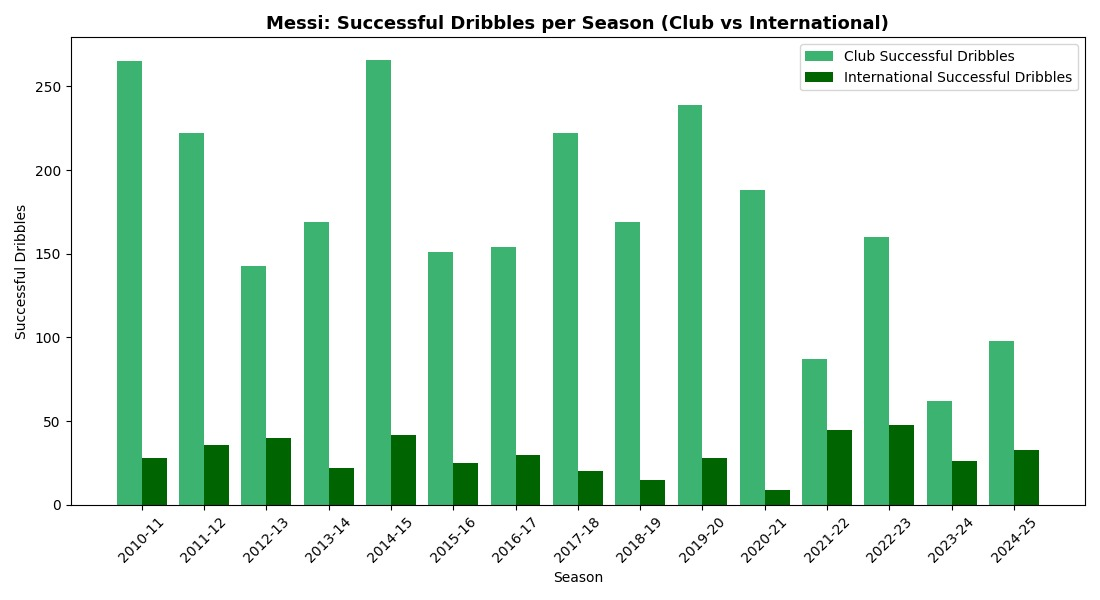
\includegraphics[width=0.9\linewidth]{WhatsApp Image 2025-11-13 at 17.06.35_3dd70965.jpg}
      \caption{}
      \label{fig:placeholder}
  \end{figure}
  This grouped bar chart, titled "Messi: Successful Dribbles per Season (Club vs International)," visualizes arguably the most physically demanding aspect of Messi's game: his ability to bypass defenders one-on-one. The vertical axis scales up to roughly 275, and the data spans from 2010-11 to 2024-25. The medium green bars (Club Successful Dribbles) highlight his explosive prime, revealing massive peaks in the 2010-11 and 2014-15 seasons where he completed over 260 dribbles. These spikes correspond to his younger years when his acceleration and agility were at their absolute zenith. While he maintained a high volume (often exceeding 150 dribbles) well into the 2019-20 season, the chart displays a sharp and undeniable decline starting in 2020-21. By the 2023-24 season, his club dribbles had dropped to below 75, a clear statistical indicator of his transition from a ball-carrying winger to a playmaking midfielder who relies more on passing than physical acceleration.

The dark green bars (International Successful Dribbles) tell a slightly different story regarding his motivation. While generally hovering between 20 and 40 dribbles per season, there is a noticeable resurgence in the 2021-22 and 2022-23 seasons, where his international dribbling output actually increased to near 50, bucking the downward trend seen in his club stats. This anomaly suggests that during Argentina's Copa América and World Cup campaigns, he forced himself to engage in more physical, solo actions for the national team, even as his body was slowing down at the club level.
    \begin{figure}[H]
      \centering
      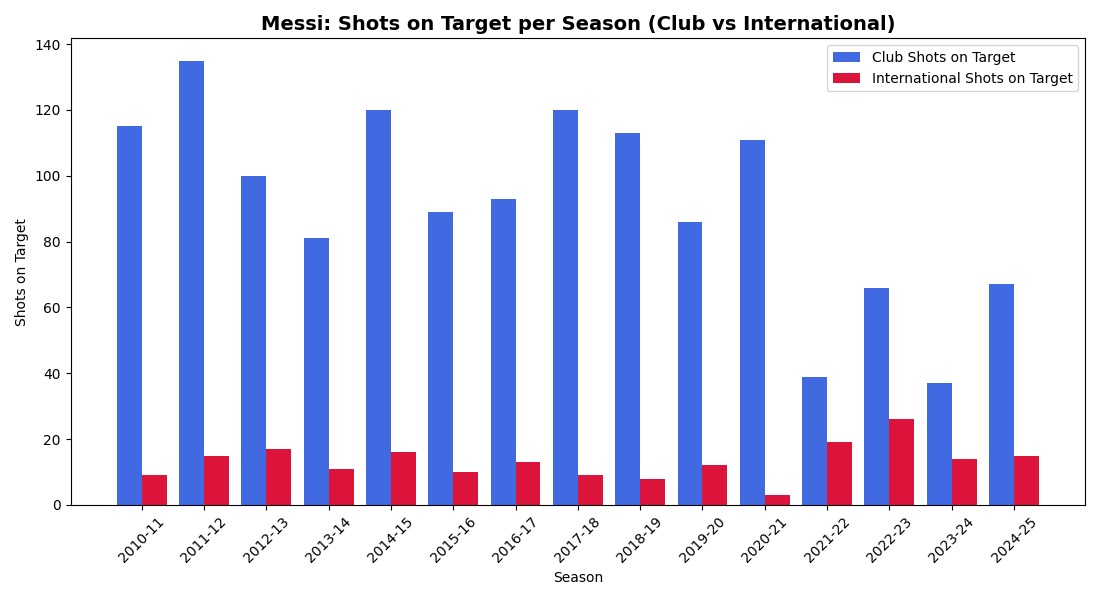
\includegraphics[width=0.9\linewidth]{WhatsApp Image 2025-11-13 at 20.15.25_19a4f257.jpg}
      \label{fig:placeholder}
  \end{figure}
  This grouped bar chart, titled "Messi: Shots on Target per Season (Club vs International)," acts as a direct measurement of Lionel Messi’s offensive aggression and threat level over the last fifteen years. The vertical axis scales up to 140, providing room to visualize his most prolific shooting years. The blue Club bars are dominated by the 2011-12 season, where he registered nearly 135 shots on target, a staggering volume that correlates perfectly with his record-breaking 73-goal season. The chart reveals a long period of sustained intensity; from 2010 through 2021, he regularly surpassed 100 shots on target per season (notably in 2014-15 and 2017-18), indicating that his role was primarily that of a high-volume finisher.

However, the visual landscape shifts dramatically in the 2021-22 season. The blue bar plummets to below 40 shots on target, marking the moment his role transitioned away from being the primary volume shooter at the club level. While there is a recovery in 2022-23 and 2024-25 (rising back to around 65-70), he never returns to the triple-digit figures of his prime. Conversely, the red International bars show a distinct career highlight in the 2022-23 season. While typically low, his international shots on target peaked at over 25 during this season, visually confirming that he saved his most aggressive shooting performances for Argentina’s World Cup-winning campaign, effectively compensating for his reduced volume at the club level.
  \begin{figure}[H]
      \centering
      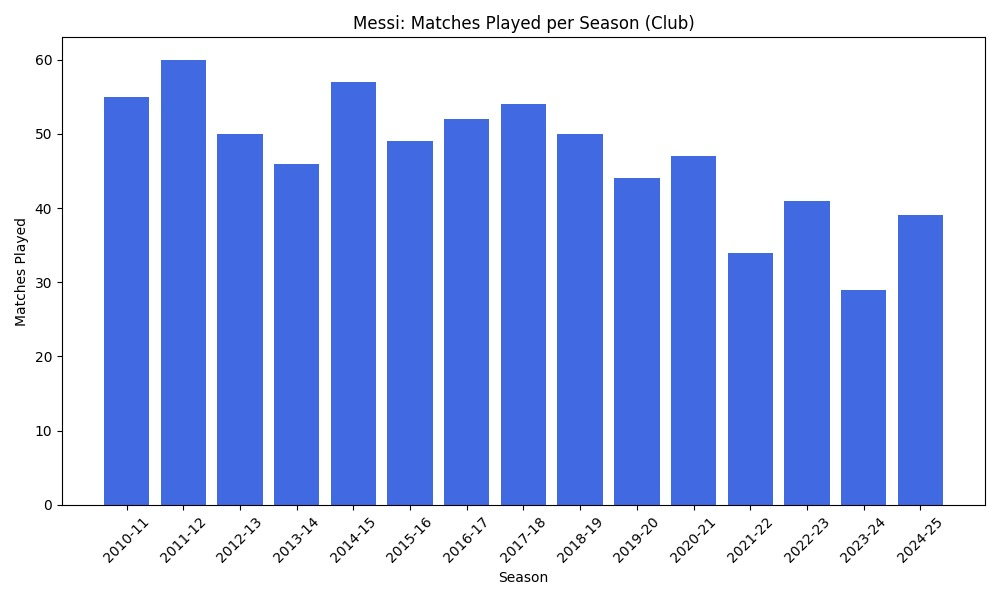
\includegraphics[width=0.9\linewidth]{WhatsApp Image 2025-11-13 at 16.39.57_2d7cc740.jpg}
      \caption{}
      \label{fig:placeholder}
  \end{figure}
  This bar chart tracks Lionel Messi’s club match appearances from the 2010-11 to 2024-25 seasons, illustrating a clear trajectory from peak durability to a managed workload in his later career. The height of the blue bars shows a maximum of 60 matches in 2011-12, gradually tapering off to 29 in 2023-24. Statistically, the distribution of this data is negatively skewed (left-skewed), meaning the vast majority of the values are concentrated at the higher end of the scale (50-60 matches), while the "tail" of the distribution is pulled downward by the lower values recorded in the most recent seasons. In terms of variability, the graph tells a tale of two eras: the first decade exhibits extremely low variance with a tight, predictable cluster of high-volume seasons, whereas the post-2020 period shows high instability and a much wider range of outcomes. Furthermore, the distribution is platykurtic (flat-topped) rather than peaked; instead of clustering sharply around a single average, the data forms a broad plateau of sustained activity, indicating that for most of his career, his "standard" performance was defined by a wide range of maximum availability rather than a narrow mean.
    \begin{figure}[H]
      \centering
      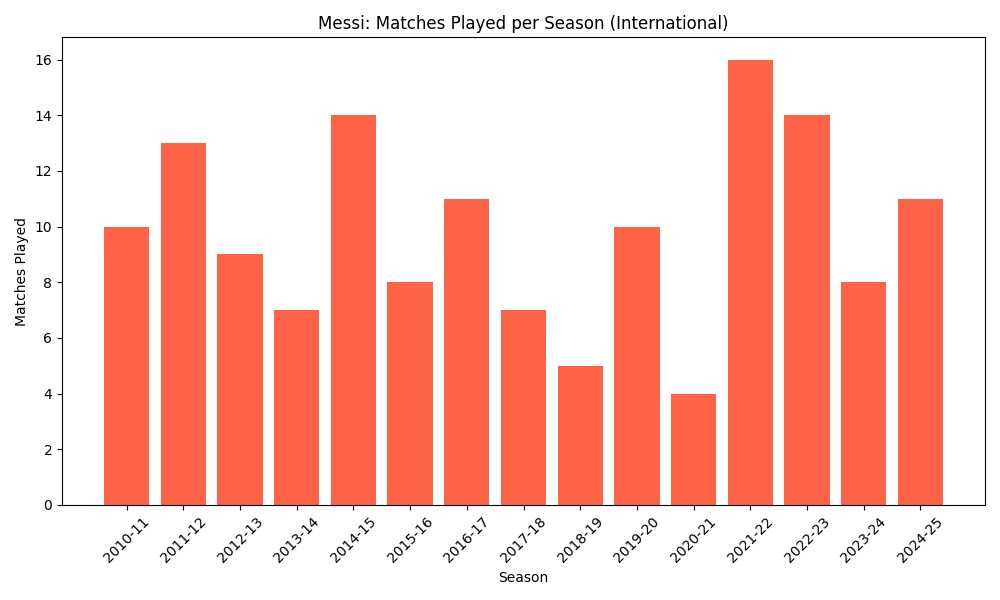
\includegraphics[width=0.9\linewidth]{WhatsApp Image 2025-11-13 at 16.40.06_9a9918e8.jpg}
      \caption{}
      \label{fig:placeholder}
  \end{figure}
This bar chart visualizes the fluctuating volume of Lionel Messi’s international appearances from 2010-11 to 2024-25, highlighting a cyclical pattern driven by major tournaments rather than a consistent league schedule. The data ranges from a pandemic-impacted low of 4 matches in 2020-21 to a career-high peak of 16 in 2021-22, underscoring the irregularity of national team duty. Statistically, this dataset exhibits high variability, contrasting sharply with the stability of his club career; the significant oscillation between peaks and troughs results in a large standard deviation relative to the mean. Unlike his club stats, the distribution shows low skewness, appearing relatively symmetrical as the data points are scattered across the entire range rather than clustering heavily at one end. Furthermore, the distribution is distinctly platykurtic (flat), lacking a sharp central peak or mode; this indicates that there is no "standard" number of international matches for Messi, but rather a uniform spread of values heavily dependent on the four-year cycles of the World Cup and Copa América.
  \begin{figure}[H]
      \centering
      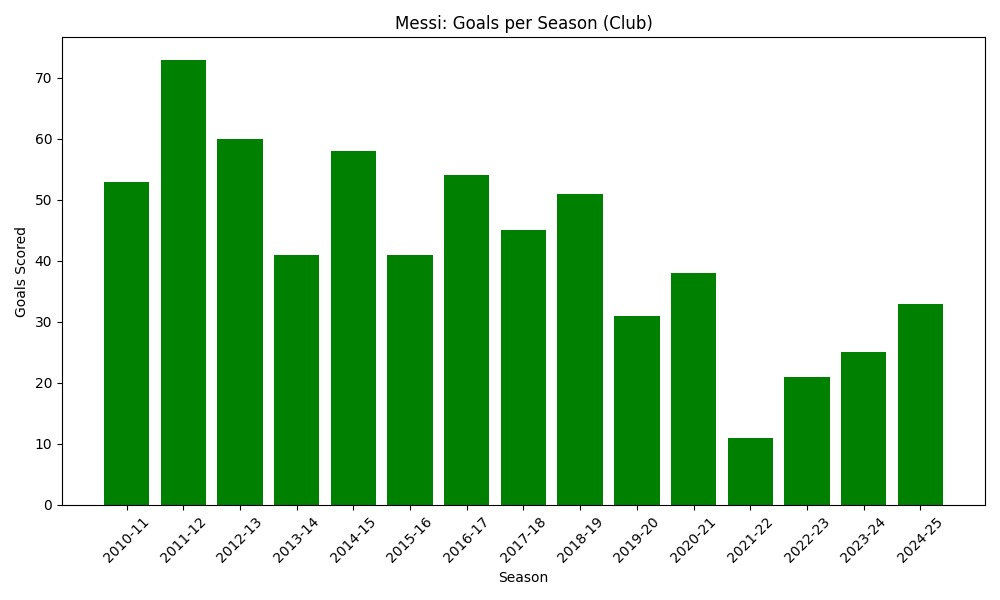
\includegraphics[width=0.9\linewidth]{WhatsApp Image 2025-11-13 at 16.13.17_bef5297a.jpg}
      \caption{}
      \label{fig:placeholder}
  \end{figure}
  This bar chart illustrates the trajectory of Lionel Messi’s club goal-scoring output from 2010-11 to 2024-25, visually dominated by his historic 2011-12 season where he netted a record-breaking 73 goals. The data reveals a decade-long period of elite production followed by a sharp decline starting in 2020-21, reaching a nadir of approximately 11 goals in 2021-22. Statistically, this dataset is defined by extremely high variability; the massive range between the peak (73) and the trough (~11) results in a large standard deviation, reflecting the drastic change in his scoring role over time. The distribution is negatively skewed (left-skewed), as the bulk of the data points cluster in the high-value region (40 to 60 goals) representing his prime years, while the "tail" of the distribution is pulled downward by the fewer, recent low-scoring seasons. Furthermore, the distribution appears platykurtic (flat); aside from the singular outlier in 2012, the data does not gather sharply around a single average but is spread broadly across a wide interval, indicating that his "standard" season varied significantly depending on his tactical role and the team's structure.
  \begin{figure}[H]
      \centering
      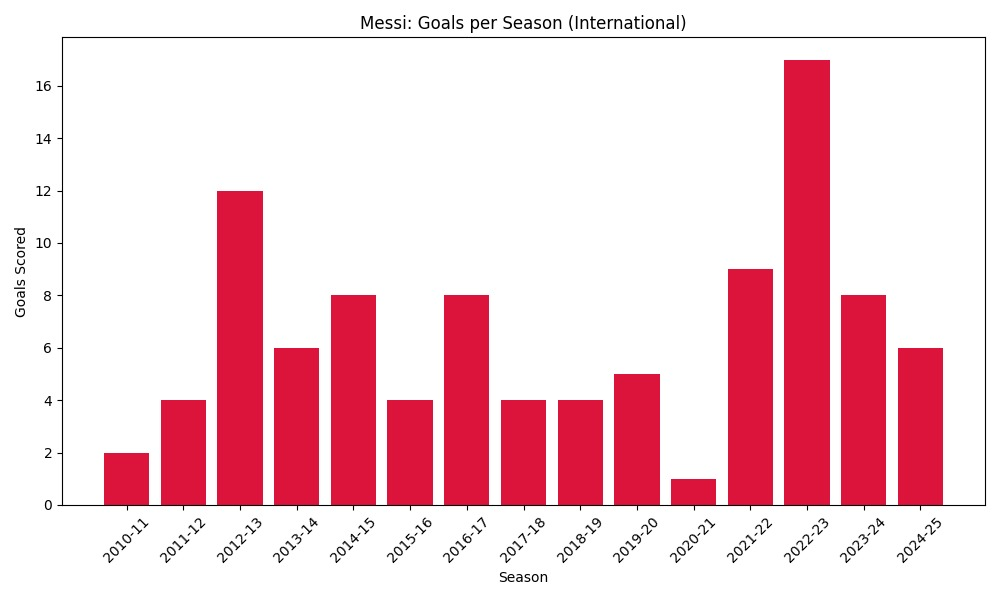
\includegraphics[width=0.9\linewidth]{WhatsApp Image 2025-11-13 at 16.18.54_8bca150c.jpg}
      \caption{}
      \label{fig:placeholder}
  \end{figure}
  This bar chart tracks the erratic nature of Lionel Messi’s goal-scoring record for the Argentina national team from 2010-11 to 2024-25. Unlike the consistent output seen in his club career, this dataset is defined by generally lower figures interspersed with dramatic surges, most notably the massive peak in the 2022-23 season where he scored nearly 18 goals. Statistically, the distribution displays positive skewness (right-skewed), which is the direct inverse of his club statistics; here, the "mass" of the data is concentrated at the lower end (typically between 2 and 8 goals), and the statistical tail is pulled upward by the positive outliers (the 12 goals in 2012-13 and the ~18 in 2022-23). The variability is exceptionally high relative to the mean, as the values fluctuate wildly from a low of just 1 goal in 2020-21 to the career-defining high in 2022-23. Furthermore, the distribution appears platykurtic (flat-topped) and irregular; there is no distinct central peak where his performance usually settles, but rather a scattered range of outcomes heavily influenced by the timing of international tournaments, resulting in "heavy tails" due to those specific high-performance outlier years.
  \begin{figure}[H]
      \centering
      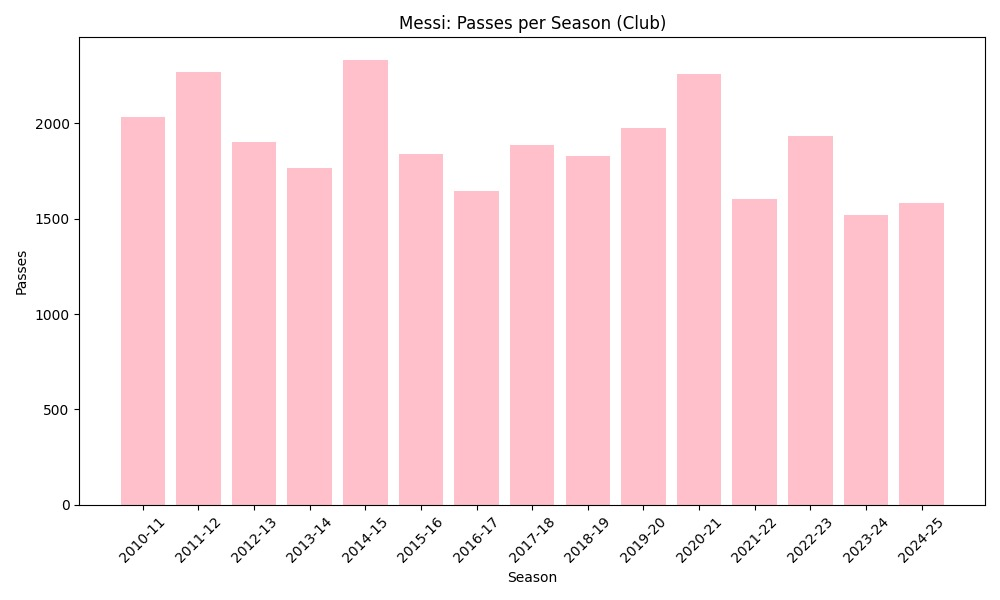
\includegraphics[width=0.9\linewidth]{WhatsApp Image 2025-11-13 at 16.20.03_a9d47f0f.jpg}
      \caption{}
      \label{fig:placeholder}
  \end{figure}
  This bar chart details the volume of Lionel Messi’s passing contributions in club football from 2010-11 to 2024-25, serving as a proxy for his involvement in play construction. The data highlights distinct peaks in the 2011-12, 2014-15, and 2020-21 seasons where his total passes exceeded 2,000, illustrating his role as the team's primary creative hub. Statistically, the distribution is negatively skewed (left-skewed), similar to his match workload; the "mass" of the data is concentrated in the higher values (typically above 1,800 passes) representing the bulk of his career, while the "tail" extends towards the lower end, driven by the noticeable decline in volume during the most recent three seasons where figures settled closer to 1,500. In terms of variability, the dataset shows moderate fluctuation; unlike his goal-scoring which saw drastic drops, his passing volume has remained relatively robust, though it has transitioned from "elite volume" to "high volume." The distribution is also platykurtic (flat-topped), as there is no single dominant mode; instead, the values are spread broadly across a 1,500–2,300 range, indicating that his level of involvement varied significantly year-to-year based on tactical instructions rather than clustering around a consistent average.
  \begin{figure}[H]
      \centering
      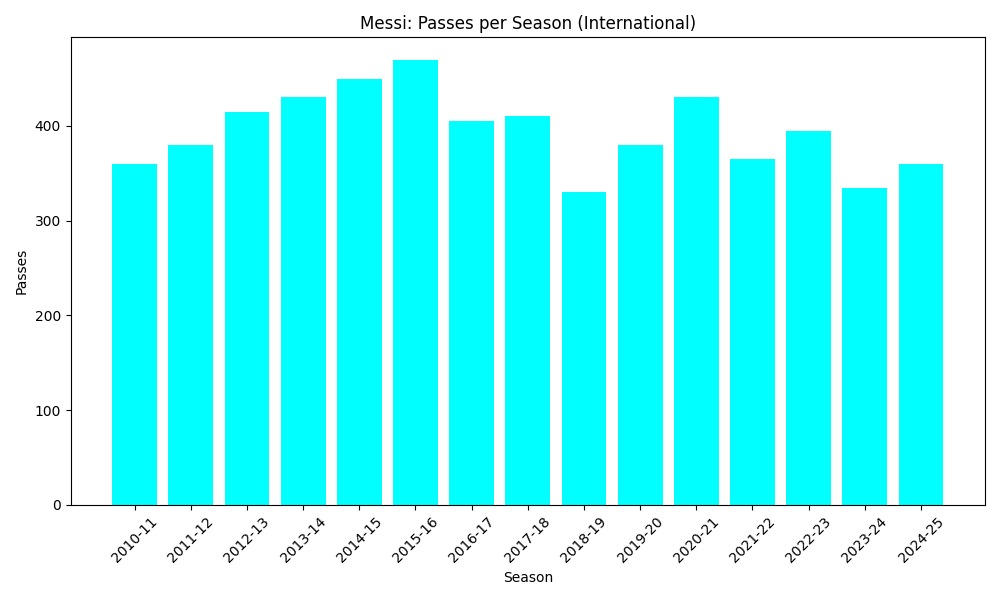
\includegraphics[width=0.9\linewidth]{WhatsApp Image 2025-11-13 at 16.26.00_fb7b1d5a.jpg}
      \caption{}
      \label{fig:placeholder}
  \end{figure}
  This bar chart visualizes the volume of passes Lionel Messi attempted for the Argentina national team from 2010-11 to 2024-25, illustrating his unwavering role as the team's primary distributor. The vertical axis ranges from 0 to over 450, showing peaks in the 2014-15 and 2020-21 seasons where he surpassed 430 passes—periods coinciding with deep Copa América runs. Statistically, this dataset exhibits low variability compared to his goal-scoring charts; the values are remarkably consistent, mostly confined within a tight range of 330 to 470 passes. This indicates that regardless of his goal output, his involvement in buildup play remained constant. The distribution is relatively symmetric (low skewness), lacking the heavy "tails" seen in his club stats, as there are no extreme outliers pulling the average significantly up or down. Furthermore, the distribution is platykurtic (flat-topped), as the data does not cluster around a single sharp peak (mode) but rather spreads evenly across a plateau of performance, suggesting that a "standard" international season for Messi consistently involved between 350 and 420 passes.
  \begin{figure}[H]
      \centering
      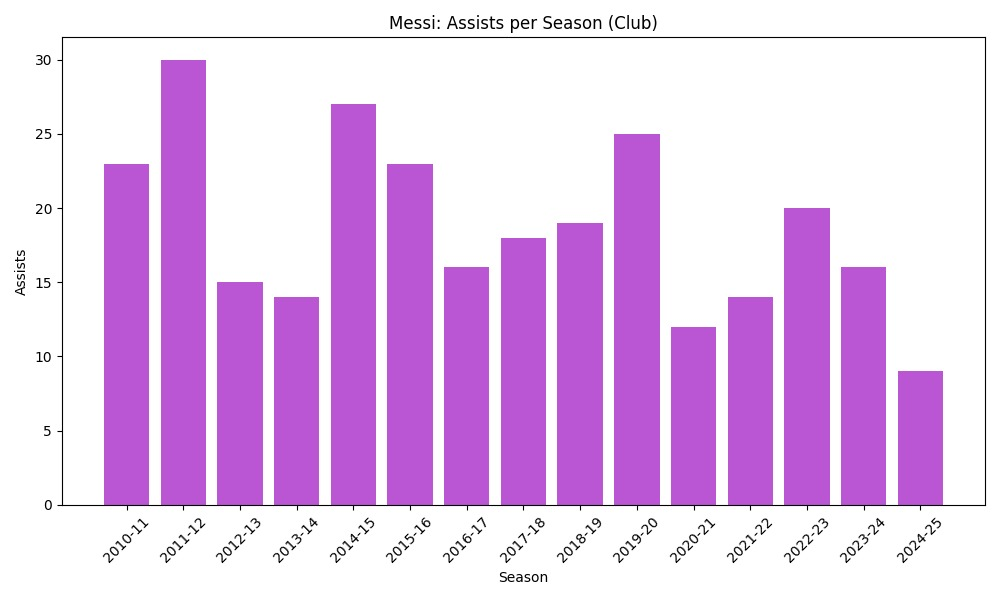
\includegraphics[width=0.9\linewidth]{WhatsApp Image 2025-11-13 at 16.36.37_9d733a4e.jpg}
      \caption{}
      \label{fig:placeholder}
  \end{figure}
  This bar chart visualizes Lionel Messi’s club assist statistics from 2010-11 to 2024-25, highlighting a career trajectory defined by periodic creative peaks rather than a steady linear trend. The purple bars reveal three distinct zeniths: a career-high 30 assists in 2011-12, followed by surges to 27 in 2014-15 and 25 in 2019-20. Statistically, this dataset exhibits high variability and a multimodal nature; unlike the steady plateau seen in his early goal-scoring, his assist numbers oscillate significantly (e.g., dropping to 15 before rocketing back to 27), reflecting his shifting tactical roles between scorer and provider. The distribution is platykurtic (flat), indicating that there is no single "normal" season for his creativity, but rather a wide dispersion of outcomes. Furthermore, the data is relatively symmetric (low skewness), as the average assist count sits centrally within the range, balanced effectively by the high outliers (30) and the recent lower values (9 in 2024-25).
  \begin{figure}[H]
      \centering
      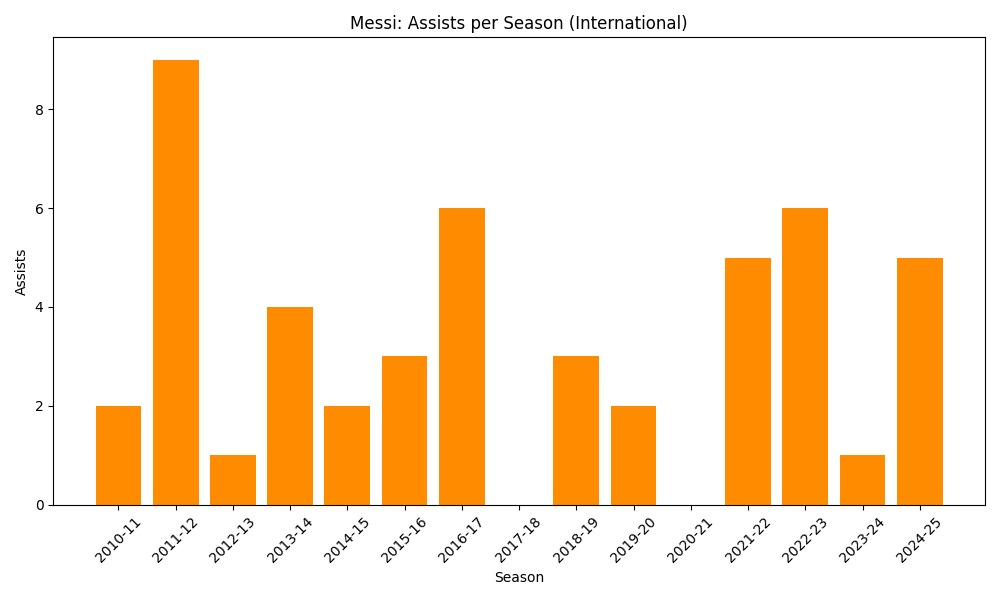
\includegraphics[width=0.9\linewidth]{WhatsApp Image 2025-11-13 at 16.36.43_d9b3815c.jpg}
      \caption{}
      \label{fig:placeholder}
  \end{figure}
  This bar chart illustrates the volatile and sporadic nature of Lionel Messi’s playmaking contributions for Argentina from 2010-11 to 2024-25, contrasting sharply with the consistency of his club metrics. The data is defined by dramatic inconsistency, featuring a solitary, massive peak of 9 assists in 2011-12, followed by a scattered pattern of secondary spikes (6 assists in 2016-17 and 2022-23) and multiple seasons with zero or near-zero output (like 2017-18 and 2020-21). Statistically, this dataset exhibits extreme variability; the standard deviation is likely very high relative to the low mean, as there is no predictable baseline for his international creativity. The distribution is positively skewed (right-skewed), as the "mass" of the data is concentrated in the low-single digits (typically 1 to 4 assists), while the singular high value of 9 pulls the statistical tail upward. Furthermore, the distribution is platykurtic (flat) and disjointed; the lack of a central peak indicates that there is no "standard" assist count for a Messi international season, but rather a series of isolated performances heavily dependent on the specific tournament context of that year.
  \begin{figure}[H]
      \centering
      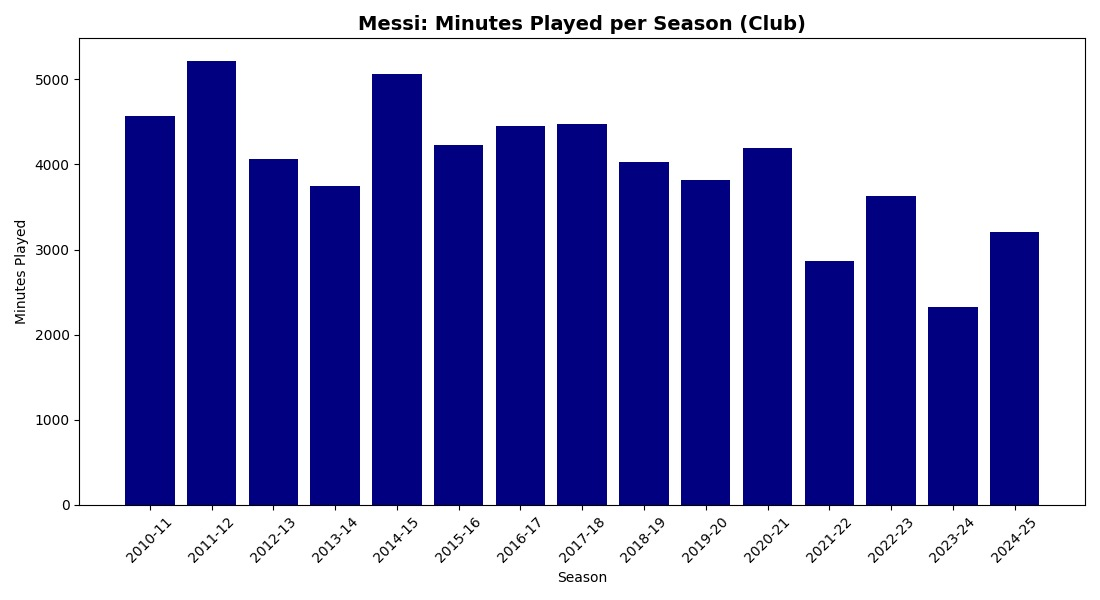
\includegraphics[width=0.9\linewidth]{WhatsApp Image 2025-11-13 at 20.09.07_de4ce722.jpg}
      \label{fig:placeholder}
  \end{figure}
  This bar chart, titled "Messi: Minutes Played per Season (Club)," serves as a quantifiable timeline of Lionel Messi’s physical endurance and availability from 2010-11 to 2024-25. The visual trajectory is defined by a decade of extreme workload—peaking above the 5,000-minute threshold in 2011-12 and 2014-15—followed by a structural decline in playing time starting in the 2021-22 season. Statistically, the distribution is negatively skewed (left-skewed); the vast majority of the data points cluster at the high end of the spectrum (between 3,800 and 5,200 minutes), establishing "elite durability" as the baseline, while the statistical tail is pulled downward by the significantly lower values of recent years (dropping to ~2,300 minutes). In terms of variability, the dataset tells a tale of two distinct eras: the period from 2010 to 2020 exhibits low variability and high predictability, where he was virtually ever-present, whereas the post-2021 era introduces high variability as his minutes fluctuate based on injury management and league transitions. Furthermore, the distribution is platykurtic (flat-topped); rather than clustering around a sharp, central average, the data forms a broad, high-volume plateau, indicating that for most of his career, his "normal" was not a specific number of minutes, but rather the maximum possible time the schedule allowed.
  \begin{figure}[H]
      \centering
      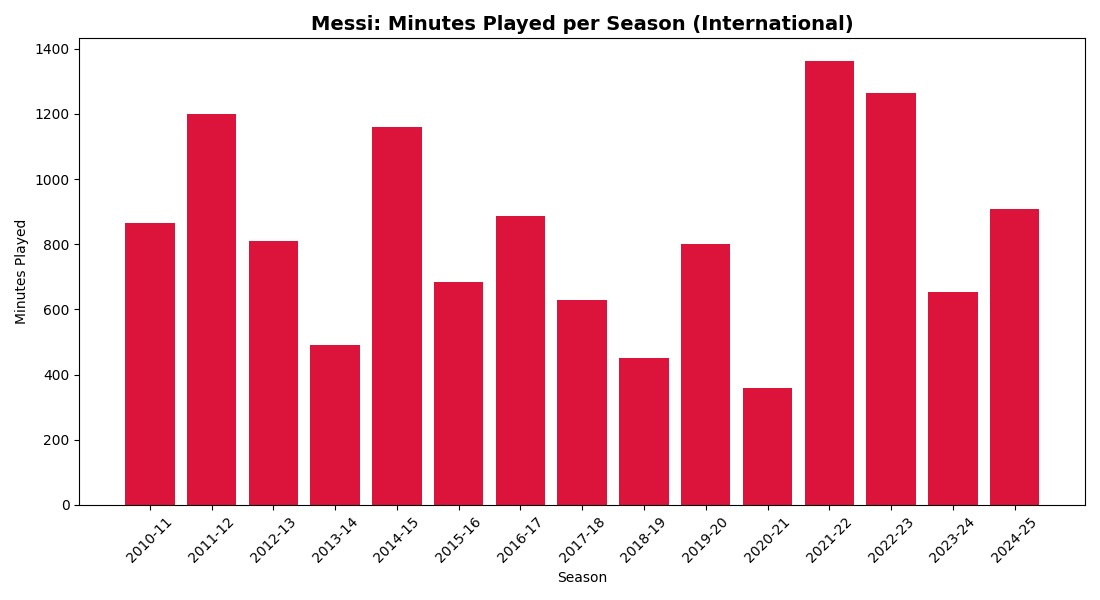
\includegraphics[width=0.9\linewidth]{WhatsApp Image 2025-11-13 at 20.09.07_8af6ce1c.jpg}
      \caption{Enter Caption}
      \label{fig:placeholder}
  \end{figure}
This bar chart visualizes the cyclical and volatile nature of Lionel Messi’s playing time for the Argentina national team from 2010-11 to 2024-25. The vertical axis scales up to 1,400 minutes, capturing the dramatic fluctuations between standard qualifying years and major tournament campaigns. The data is dominated by two major peaks: the 2011-12 season and the all-time high in 2021-22, where he played nearly 1,400 minutes, reflecting the intense schedule surrounding Argentina's Copa América and World Cup success. Statistically, this dataset exhibits high variability, characterized by sharp oscillations between these peaks and deep troughs (such as the pandemic-shortened 2020-21 season with only ~360 minutes). Unlike his club duration, which was negatively skewed, this distribution shows low skewness and appears relatively symmetric; high-volume seasons and low-volume seasons are scattered somewhat evenly across the timeline rather than clustering at one end. Furthermore, the distribution is platykurtic (flat and multimodal), lacking a single central mode; this statistical flatness confirms that there is no "standard" workload for Messi internationally, but rather a binary outcomes determined entirely by how deep Argentina progressed in summer tournaments.
    \begin{figure}[H]
      \centering
      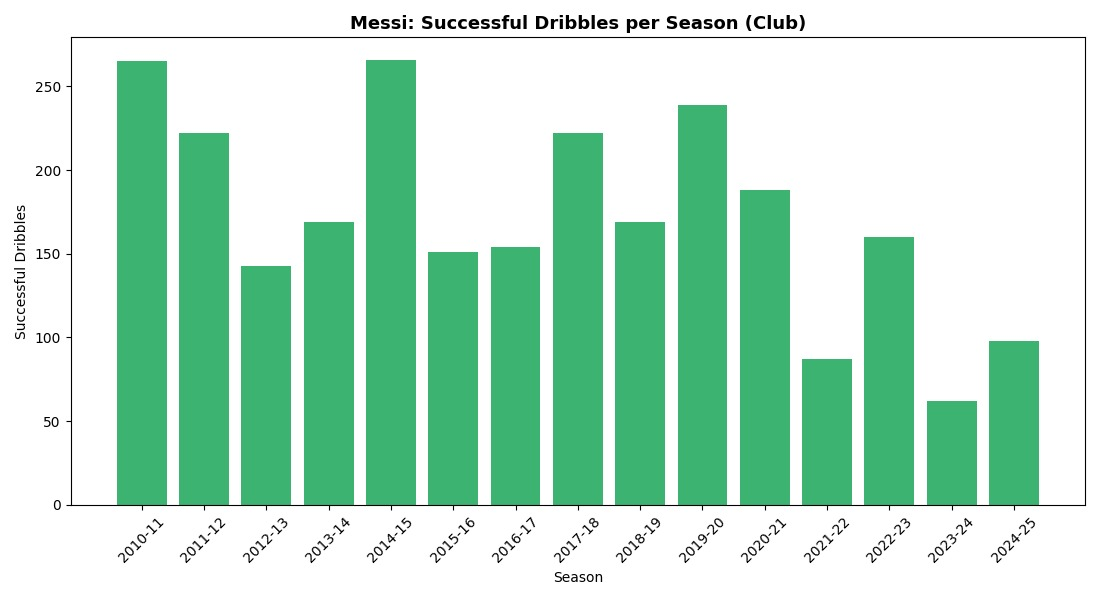
\includegraphics[width=0.9\linewidth]{WhatsApp Image 2025-11-13 at 17.06.44_8b459166.jpg}
      \caption{}
      \label{fig:placeholder}
  \end{figure}
  This bar chart tracks the trajectory of Lionel Messi’s successful dribbles in club football from 2010-11 to 2024-25, offering the clearest statistical evidence of his physical evolution. The data reveals a distinct "era of dominance" between 2010 and 2020, where he frequently surpassed 200 successful dribbles per season, with massive peaks in 2010-11 and 2014-15 (reaching nearly 270). This period defines him as a high-volume ball carrier. However, a sharp structural break occurs in the 2021-22 season, where the volume drops below 100 for the first time, hitting a career low of roughly 60 in 2023-24.

Statistically, this dataset is defined by high variability, as the values span a massive range from 265 down to 60, resulting in a large standard deviation that reflects the diminishing returns of age on physical agility. The distribution is negatively skewed (left-skewed); the "mass" of the data is heavily concentrated in the high-value region (150–250 dribbles) representing the majority of his career, while the statistical "tail" is pulled downward by the outliers of the last three seasons. Furthermore, the distribution is platykurtic (flat), lacking a sharp central peak. Instead of clustering around a consistent average, the data is spread broadly across the spectrum, indicating that his dribbling output was never static but rather a fluctuating metric that declined in stages as his role shifted from a winger to a playmaker.
  \begin{figure}[H]
      \centering
      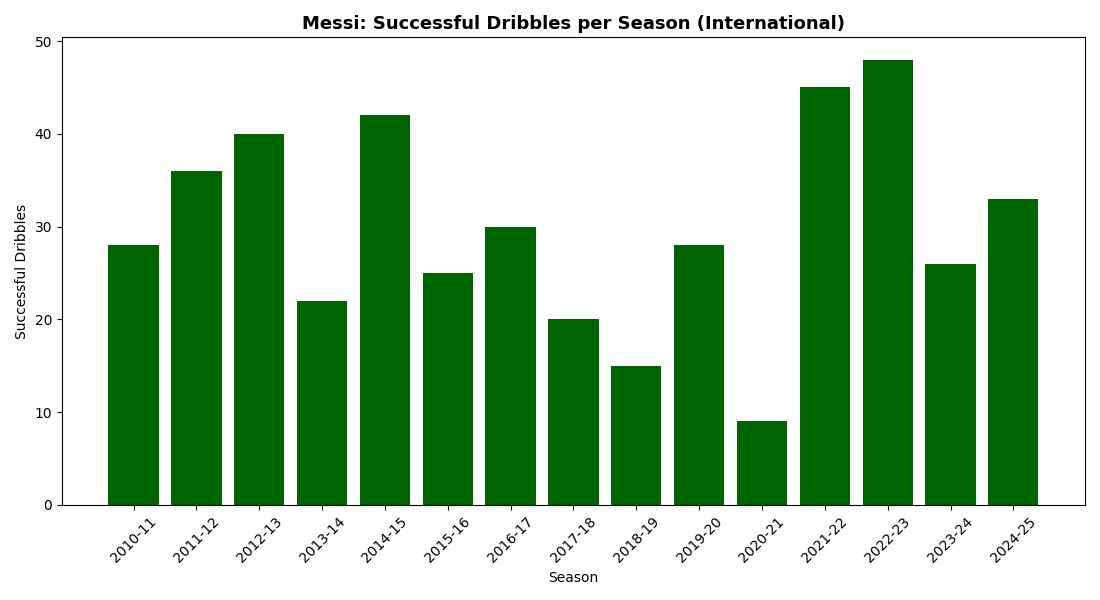
\includegraphics[width=0.9\linewidth]{WhatsApp Image 2025-11-13 at 17.06.56_68d968c7.jpg}
      \caption{}
      \label{fig:placeholder}
  \end{figure}
  This bar chart illustrates the unique trajectory of Lionel Messi’s dribbling output for the Argentina national team from 2010-11 to 2024-25, presenting a trend that stands in stark contrast to his club statistics. While his club dribbling numbers declined significantly with age, this dataset reveals a remarkable "late-career bloom," with the highest peaks occurring in the 2021-22 (~45 dribbles) and 2022-23 (~48 dribbles) seasons. This suggests that during Argentina's World Cup winning era, he assumed a more physically aggressive, ball-carrying role despite being in his mid-30s. Statistically, this dataset exhibits extremely high variability, as the values oscillate wildly between the pandemic-impacted low of roughly 9 dribbles in 2020-21 and the career-high of nearly 50 just two years later. Unlike the negatively skewed club charts, this distribution displays low skewness (relative symmetry); the data is balanced between early career highs, mid-career dips, and late-career resurgences, rather than clustering at one end. Furthermore, the distribution is platykurtic (flat and multimodal), indicating that there is no "standard" dribbling baseline for his international career; instead, the output was dictated entirely by the specific tactical necessities of each tournament cycle, resulting in a scattered and unpredictable statistical profile.
    \begin{figure}[H]
      \centering
      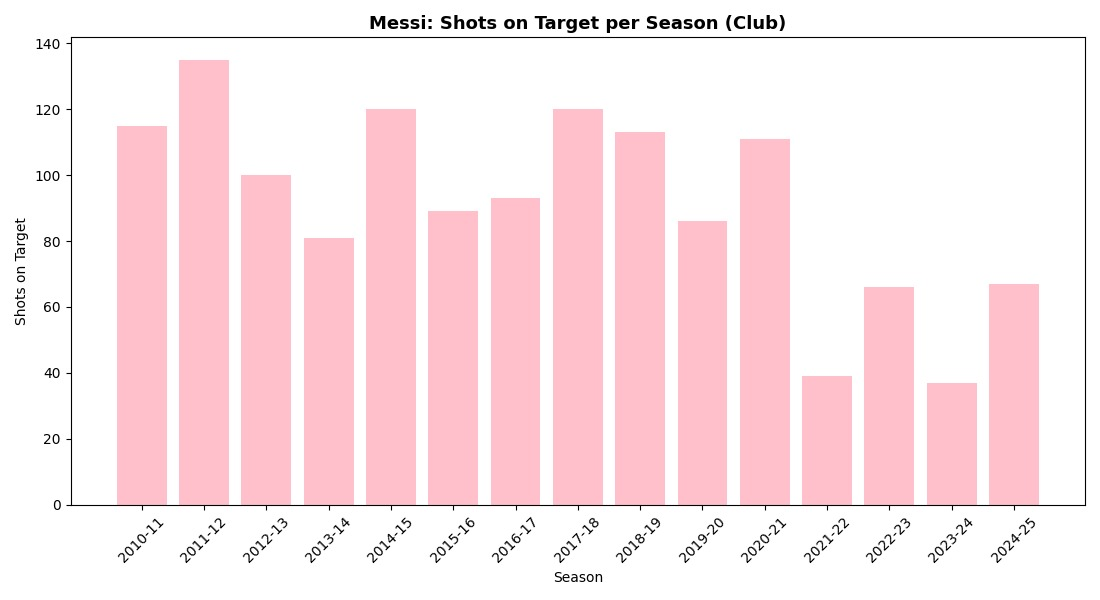
\includegraphics[width=0.9\linewidth]{WhatsApp Image 2025-11-13 at 20.20.36_c8950e2f.jpg}
      \label{fig:placeholder}
  \end{figure}
  This bar chart tracks the volume of Lionel Messi’s shots on target in club football from 2010-11 to 2024-25, serving as a direct metric of his offensive aggression and finishing threat. The visual is dominated by a decade-long plateau of high intensity, where he consistently registered between 90 and 135 shots on target, peaking in the historic 2011-12 season. This era reflects his role as the primary terminus of his team's attack. However, a distinct structural break appears in the 2021-22 season, where the volume plummets to roughly 40, reflecting a shift to a deeper playmaking role and a league change. Statistically, the dataset is characterized by high variability; the massive range between the peak (135) and the recent lows (~38) creates a large standard deviation, indicative of a player whose output has undergone a fundamental transformation. The distribution is negatively skewed (left-skewed), as the "mass" of the data is heavily concentrated at the high end of the scale (representing his prime years), while the statistical tail is pulled downward by the fewer, recent low-volume seasons. Furthermore, the distribution is platykurtic (flat-topped); rather than clustering sharply around a single average, the data spreads broadly across a high-volume range, suggesting that for the majority of his career, his "standard" was simply an elite level of offensive production that varied based on the team's specific tactical setup.
  \begin{figure}[H]
      \centering
      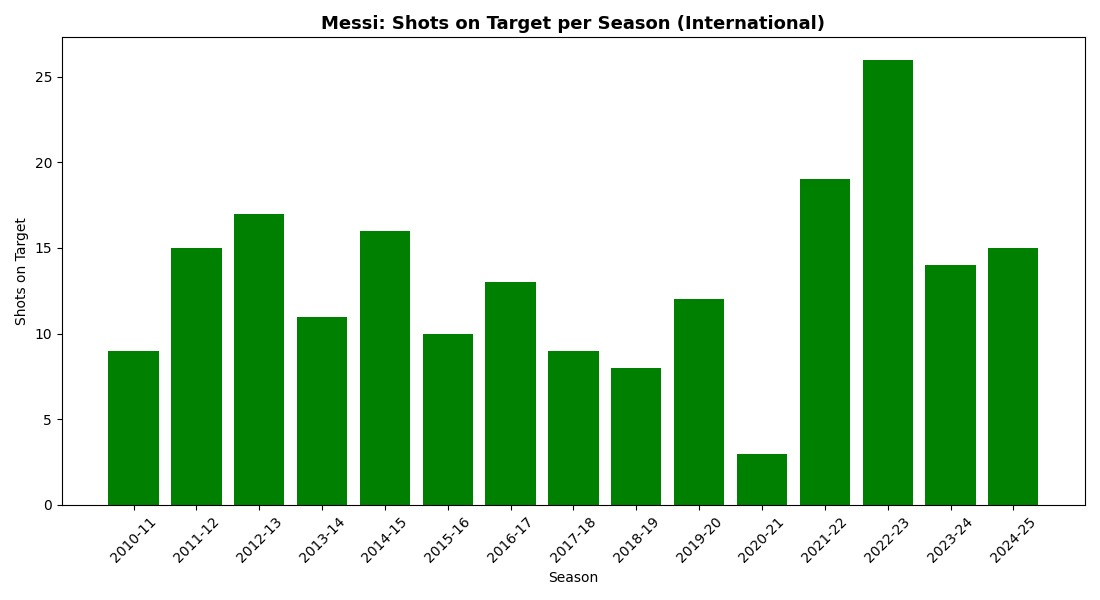
\includegraphics[width=0.9\linewidth]{WhatsApp Image 2025-11-13 at 20.14.23_e01dc3af.jpg}
      \label{fig:placeholder}
  \end{figure}
This bar chart visualizes the offensive aggression of Lionel Messi for the Argentina national team from 2010-11 to 2024-25, highlighting a fascinating inversion of his club career trajectory. While his club output generally declined in later years, this dataset reveals a massive, career-defining surge in his mid-30s. The visual is dominated by the 2022-23 season, where he registered an all-time high of over 25 shots on target, coinciding with his World Cup victory. This peak towers over his earlier years, where he typically hovered between 8 and 17 shots. Statistically, this dataset exhibits high variability, characterized by sharp fluctuations—such as the drop to a mere 3 shots in the pandemic-impacted 2020-21 season followed immediately by the rapid ascent to his career peak. The distribution is positively skewed (right-skewed); unlike his club stats (where the "mass" was at the high end), here the bulk of the data sits in the lower-to-moderate range (10-15 shots), and the statistical tail is pulled upward by the outlier performance of his World Cup campaign. Furthermore, the distribution is platykurtic (flat), as there is no single central mode where his performance settles; instead, the data is scattered broadly, reflecting that his international offensive threat was highly dependent on the specific tournament calendar of each year.


    \begin{figure}[H]
      \centering
      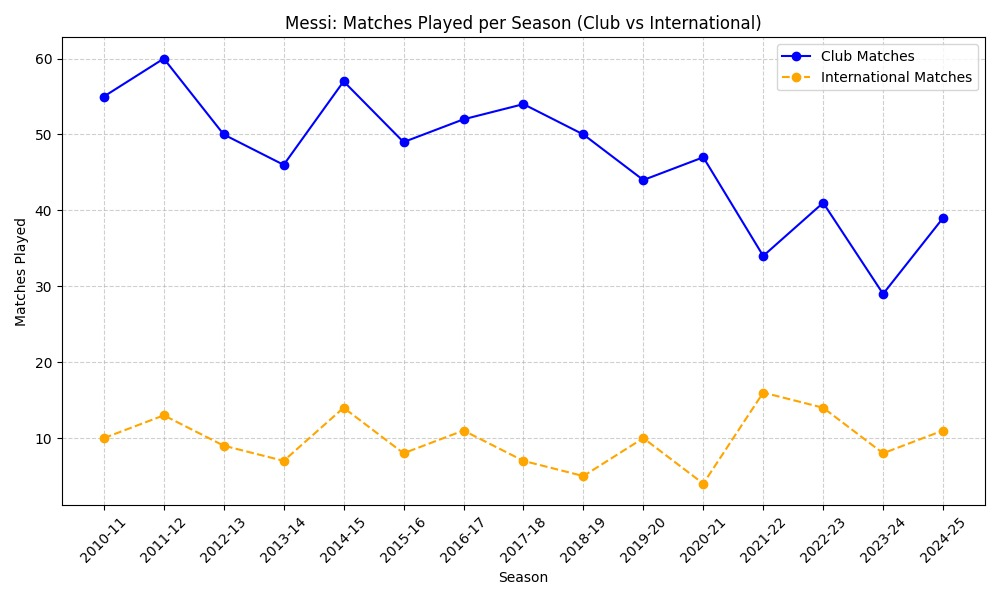
\includegraphics[width=0.9\linewidth]{WhatsApp Image 2025-11-13 at 16.44.07_38dbd0c1.jpg}
      \caption{}
      \label{fig:placeholder}
  \end{figure}
  The line plot compares Messi’s matches played per season for club and international competitions from 2010--11 to 2024--25. The data clearly shows that club match counts are consistently much higher, usually ranging between 34 and 60 matches per season, with notable peaks in 2011--12 and 2014--15. In contrast, international match counts remain substantially lower, typically fluctuating between 4 and 16 matches per season, with occasional increases in years such as 2014--15 and 2021--22. Both trends exhibit seasonal variation, yet the gap between club and international match involvement remains wide throughout the entire period. Overall, the plot highlights Messi’s significantly greater participation in club fixtures compared to international competitions.

  \begin{figure}[H]
      \centering
      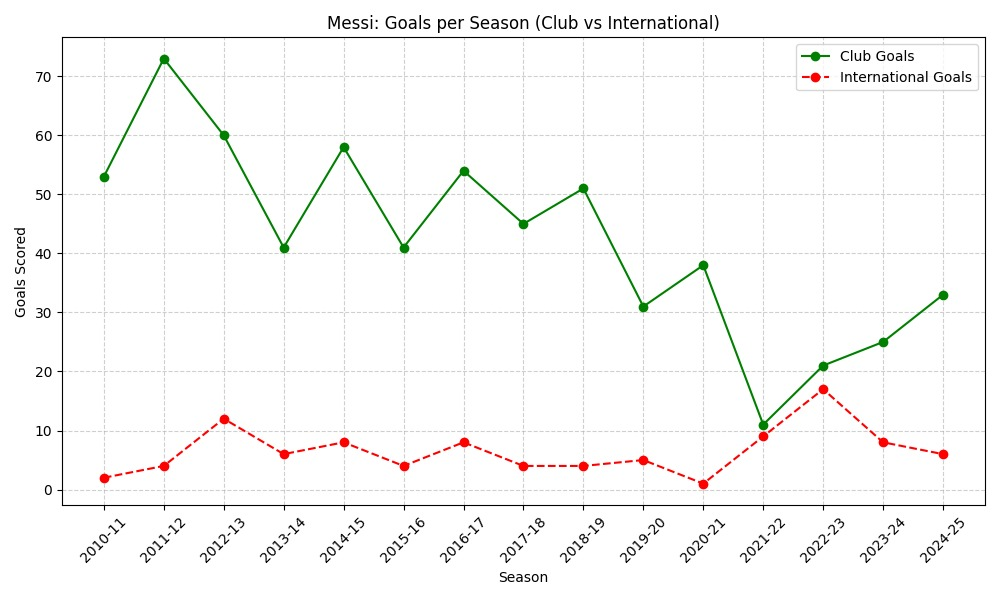
\includegraphics[width=0.9\linewidth]{WhatsApp Image 2025-11-13 at 16.44.14_5b9f8580.jpg}
      \caption{}
      \label{fig:placeholder}
  \end{figure}
  The line plot compares Messi’s goals per season for club and international competitions from 2010--11 to 2024--25. The data shows a substantial and consistent gap between the two levels, with club goals far exceeding international goals throughout the entire period. Club performance varies across seasons, ranging from peaks such as 73 goals in 2011--12 to lower outputs around 11 goals in 2021--22, yet remains significantly higher overall. International goals follow a much smaller range, typically between 1 and 12 goals per season, with occasional increases in seasons like 2012--13 and 2022--23. Although both datasets fluctuate over time, the persistent disparity demonstrates Messi’s considerably higher goal-scoring output at the club level compared to international play. Overall, the plot highlights a strong and stable dominance of club performance in terms of goals scored.

  
  \begin{figure}[H]
      \centering
      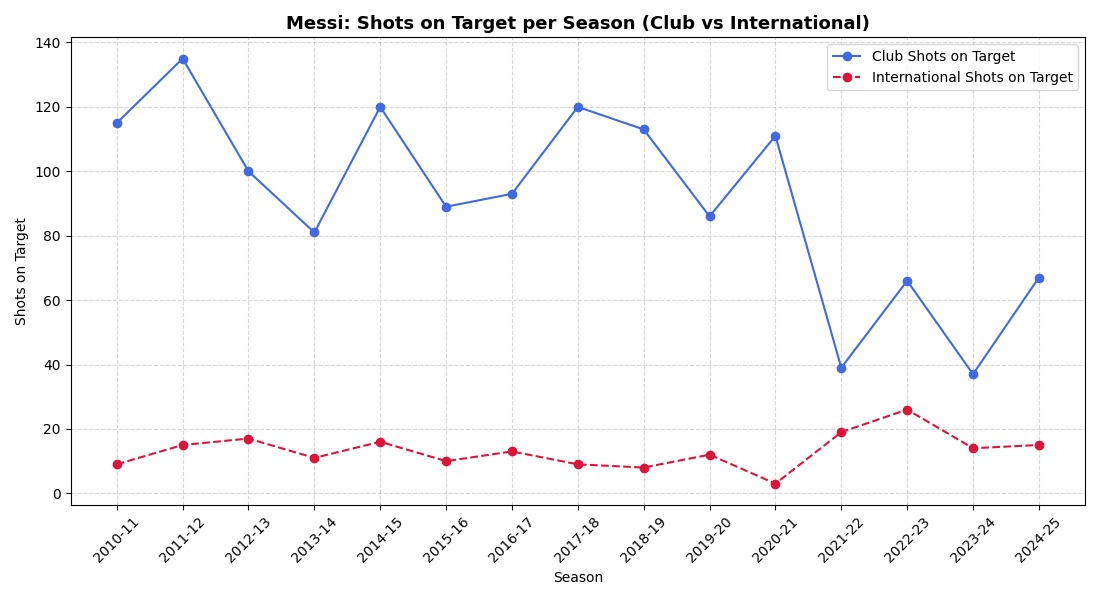
\includegraphics[width=0.9\linewidth]{WhatsApp Image 2025-11-13 at 17.13.28_b9166d9b.jpg}
      \caption{}
      \label{fig:placeholder}
  \end{figure}
  The line plot compares Messi’s shots on target per season for both club and international competitions from 2010--11 to 2024--25. The data shows a clear and consistent disparity, with club shots on target vastly exceeding international figures across all seasons. Club performance fluctuates notably, ranging from around 38 to 135 shots on target, with pronounced peaks in seasons such as 2011--12 and 2017--18. In contrast, international shots on target remain comparatively low, generally falling between 3 and 26 per season, with occasional small spikes in seasons like 2021--22 and 2022--23. Despite seasonal variation, the gap stays large and persistent. Overall, the analysis demonstrates that Messi produces significantly more shots on target at the club level than in international play, reflecting greater attacking involvement in club competitions.

  \begin{figure}[H]
      \centering
      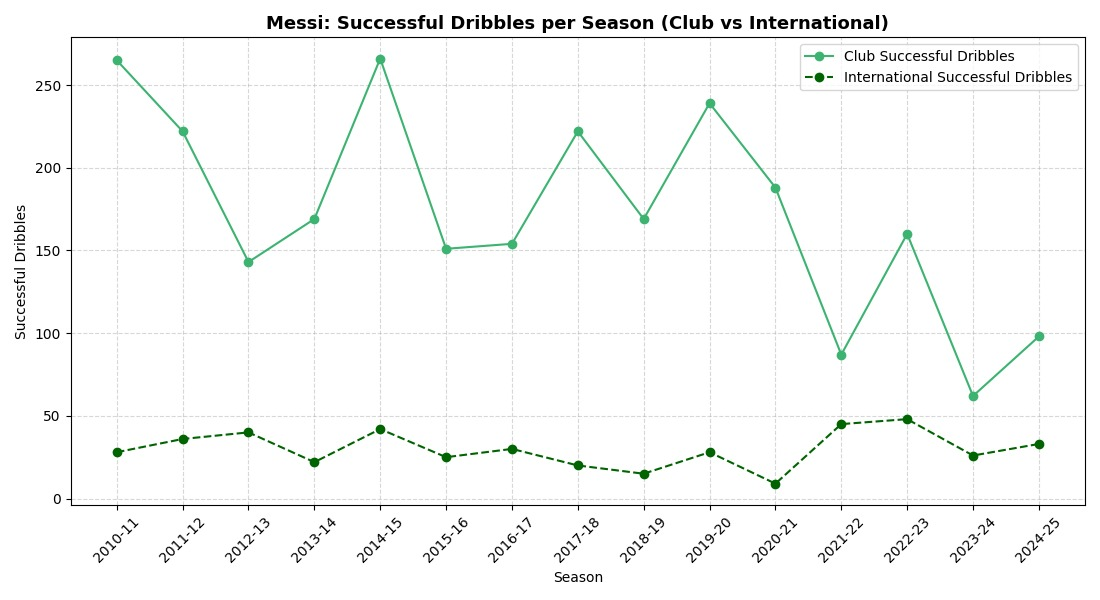
\includegraphics[width=0.9\linewidth]{WhatsApp Image 2025-11-13 at 17.13.37_a9dec154.jpg}
      \caption{}
      \label{fig:placeholder}
  \end{figure}
  The line plot compares Messi’s successful dribbles per season for club and international competitions from 2010--11 to 2024--25. The results show a consistently large gap between the two levels, with club dribbles far exceeding international dribbles across all seasons. Club dribbling performance fluctuates significantly, ranging roughly between 90 and 270 successful dribbles, with pronounced peaks in seasons such as 2010--11, 2014--15, and 2019--20. In contrast, international dribbles remain relatively low and stable, generally falling between 10 and 50 per season. Despite year-to-year variability, the persistent disparity demonstrates that Messi performs substantially more successful dribbles at the club level than in international play, highlighting a consistently higher dribbling output in club competitions.

  \begin{figure}[H]
      \centering
      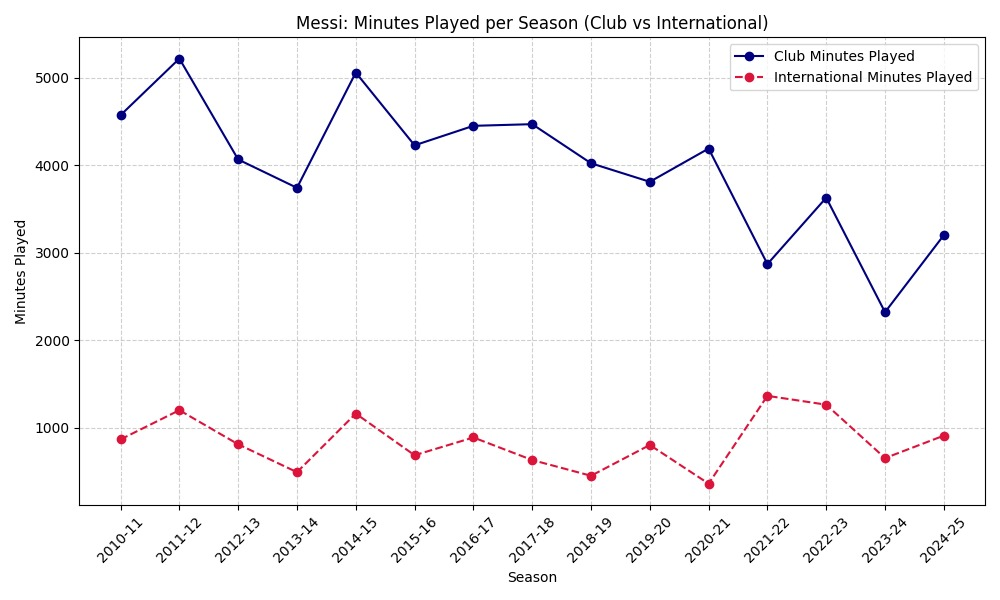
\includegraphics[width=0.9\linewidth]{WhatsApp Image 2025-11-13 at 20.25.50_a2eea4ba.jpg}
      \label{fig:placeholder}
  \end{figure}
  The line plot compares Messi’s minutes played per season at the club and international levels from 2010--11 to 2024--25. The data shows that club minutes are consistently and substantially higher, typically ranging between 3,000 and 5,200 minutes per season. International minutes are much lower, generally fluctuating between 400 and 1,300 minutes. Both trends exhibit year-to-year variability, with notable peaks such as 2011--12 and 2014--15 for club minutes, and 2011--12 and 2021--22 for international minutes. Despite these fluctuations, the gap between club and international playing time remains large and persistent throughout the observed period. Overall, the analysis highlights Messi’s heavier match involvement at the club level compared to international competitions.


  \begin{figure}[H]
      \centering
      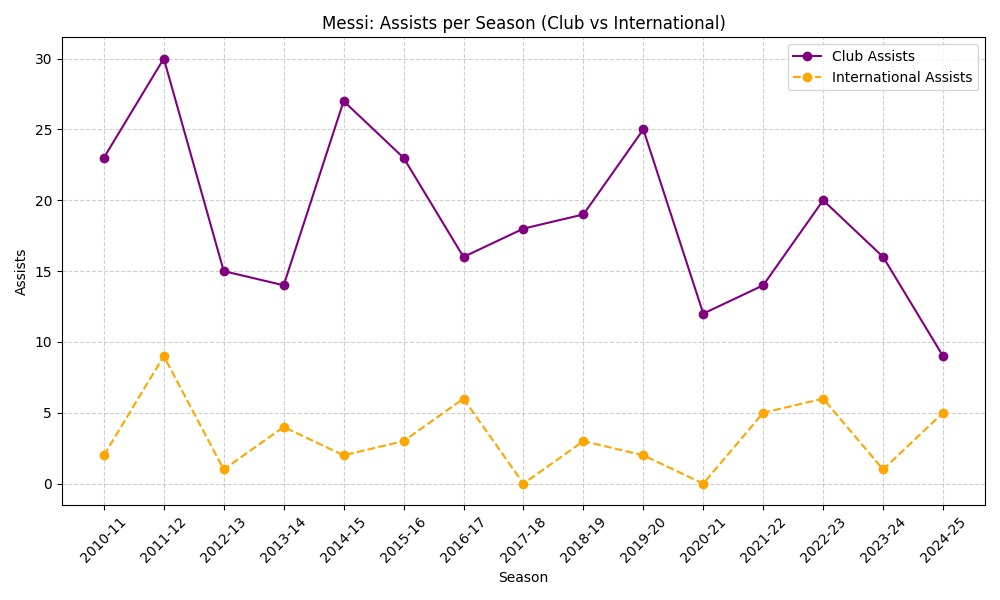
\includegraphics[width=0.9\linewidth]{WhatsApp Image 2025-11-13 at 20.25.51_9de03e6a.jpg}
      \caption{}
      \label{fig:placeholder}
  \end{figure}
  The line plot compares Messi’s assists per season for club and international competitions from 2010--11 to 2024--25. The data reveals that club assists consistently exceed international assists by a wide margin across all seasons. Club performance shows noticeable fluctuations, with peaks such as 30 assists in 2011--12 and 27 assists in 2014--15, alongside declines in later seasons. In contrast, international assists remain relatively low and stable, generally ranging between 0 and 6 each season. Although both trends show year-to-year variability, the gap between club and international assists remains persistent. Overall, the analysis highlights Messi’s significantly higher creative output at the club level compared to his international performances.

  \begin{figure}[H]
      \centering
      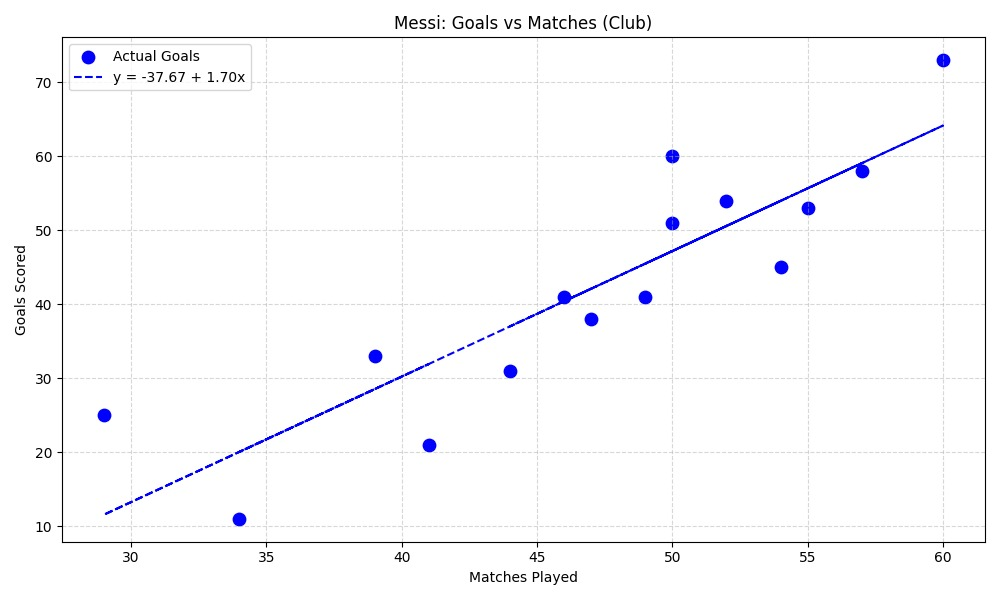
\includegraphics[width=0.9\linewidth]{WhatsApp Image 2025-11-13 at 18.03.30_936343a6.jpg}
      \caption{
      Correlation(r)=0.8838706849608278
      }
      \label{fig:placeholder}
  \end{figure}
  The scatter plot illustrates the relationship between Messi’s goals scored and matches played at the club level. The data points form a clear upward trend, indicating that goal output increases steadily as the number of matches rises. The regression line, with a positive slope of approximately $1.70$, suggests that each additional match corresponds to nearly two more goals on average. The correlation coefficient, which is strongly positive at $r = 0.884$, confirms a high degree of linear association between the two variables. Overall, the analysis demonstrates that Messi’s goal-scoring performance at the club level is closely and consistently linked to his match participation, reflecting a strong and reliable relationship.


  \begin{figure}[H]
      \centering
      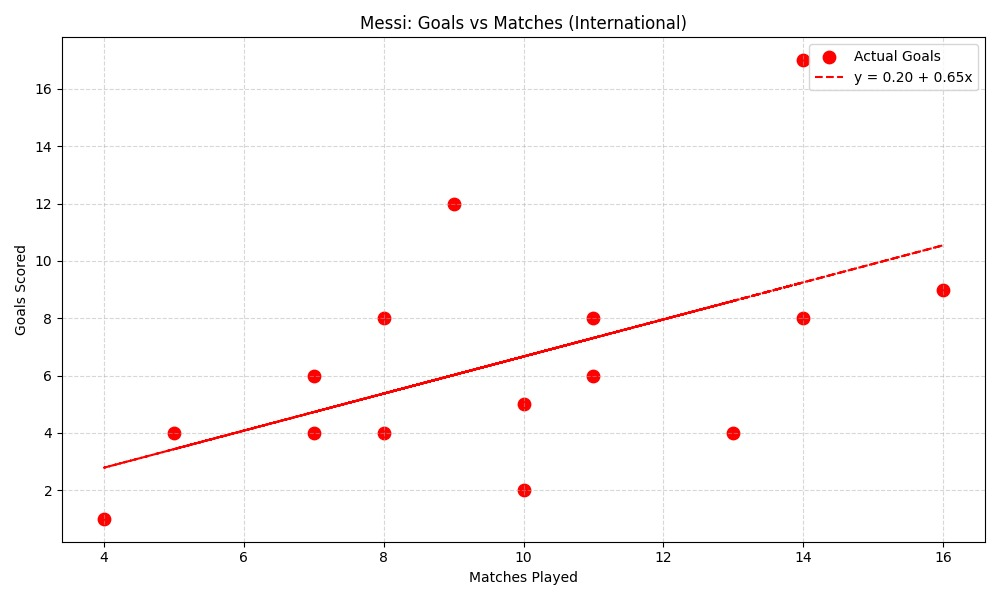
\includegraphics[width=0.9\linewidth]{WhatsApp Image 2025-11-13 at 18.03.38_3cc47357.jpg}
      \caption{Correlation(r)=0.5442400752092061}
      \label{fig:placeholder}
  \end{figure}
  The scatter plot illustrates the relationship between Messi's goals scored and matches played in international competitions. The data shows a mild upward trend, indicating that goal totals tend to increase with more match appearances, although the spread of points suggests considerable variability. The regression line has a modest positive slope of approximately $0.65$, implying that each additional match contributes less than one goal on average. The correlation coefficient of $r = 0.544$ indicates a moderate positive relationship between the variables. Overall, while the association is present, the analysis shows that Messi’s international goal-scoring displays noticeable fluctuation and is only moderately linked to the number of matches played.

  
  
  \begin{figure}[H]
      \centering
      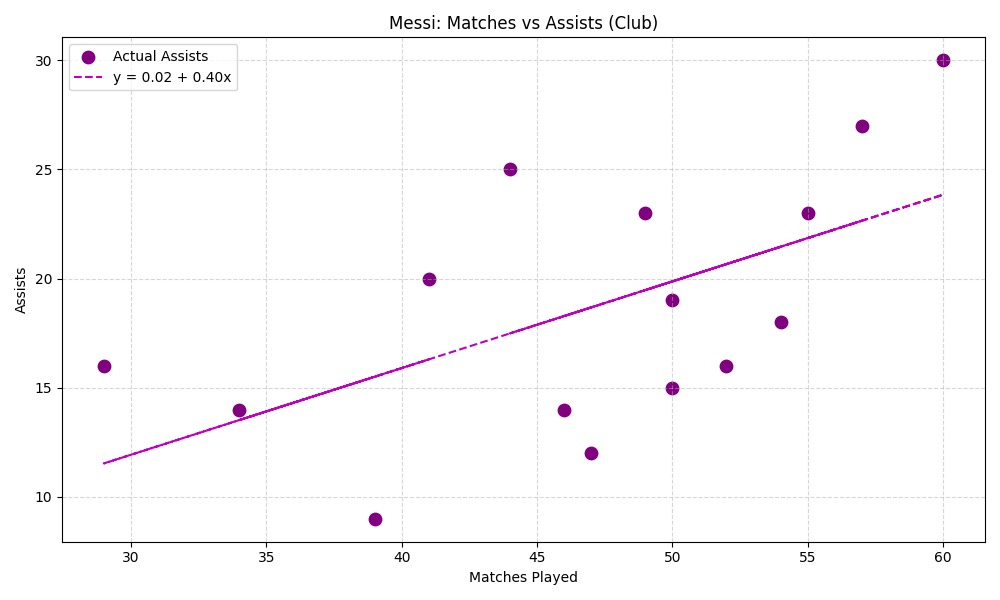
\includegraphics[width=0.9\linewidth]{WhatsApp Image 2025-11-13 at 18.03.46_5a8bd19d.jpg}
      \caption{Correlation(r)=0.5777909997178216}
      \label{fig:placeholder}
  \end{figure}
  The scatter plot illustrates the relationship between Messi’s assists and matches played at the club level. The data shows a mildly increasing trend, suggesting that assist numbers tend to rise as match participation increases, although with noticeable variability. The regression line, with a slope of approximately $0.40$, indicates that each additional match contributes less than one extra assist on average. The correlation coefficient of $r = 0.5778$ reflects a moderate positive linear relationship, meaning the association is present but not very strong. Overall, the analysis shows that while Messi’s club assists generally increase with more matches played, the relationship is moderate and influenced by fluctuations in seasonal performance.

    
  \begin{figure}[H]
      \centering
      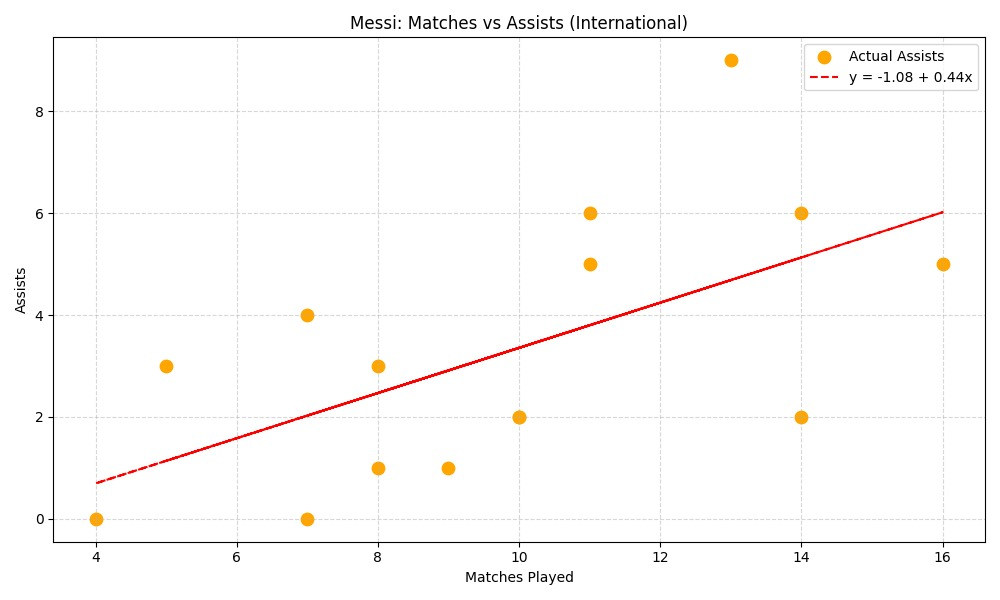
\includegraphics[width=0.9\linewidth]{WhatsApp Image 2025-11-13 at 18.03.54_7125611b.jpg}
      \caption{Correlation(r)=0.58723935936639}
      \label{fig:placeholder}
  \end{figure}
  The scatter plot illustrates the relationship between Messi's assists and matches played in international competitions. The data shows a generally upward trend, indicating that assists tend to increase as the number of matches rises, although with noticeable variability. The regression line, with a modest positive slope of approximately $0.44$, suggests that each additional match contributes less than one additional assist on average. The correlation coefficient of $r = 0.587$ indicates a moderate positive relationship between the two variables. Overall, while the association is not very strong, the analysis shows that Messi’s assist numbers tend to grow gradually with increased match participation at the international level.
  
  \begin{figure}[H]
      \centering
      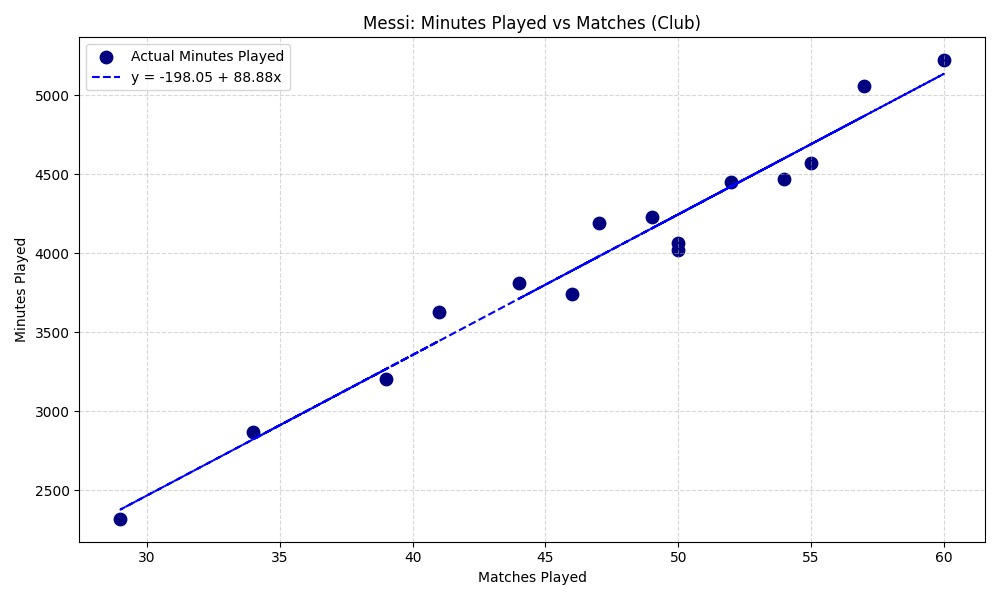
\includegraphics[width=0.9\linewidth]{WhatsApp Image 2025-11-13 at 18.04.02_4f4a733c.jpg}
      \caption{  
      Correlation(r)=0.9830690922885921}
      \label{fig:placeholder}
  \end{figure}
The scatter plot displays the relationship between Messi's minutes played and matches played at the club level. The points align closely along an upward-sloping trend line, indicating that total minutes played increase consistently with the number of match appearances. The regression line, with a slope of approximately $88.88$, suggests that each additional match contributes nearly eighty-nine more minutes on average. The very high correlation coefficient of $r = 0.983$ confirms an exceptionally strong linear relationship between the two variables. Overall, the analysis shows that Messi's club-level playing time is almost perfectly predicted by the number of matches he participates in.
  
  

  \begin{figure}[H]
      \centering
      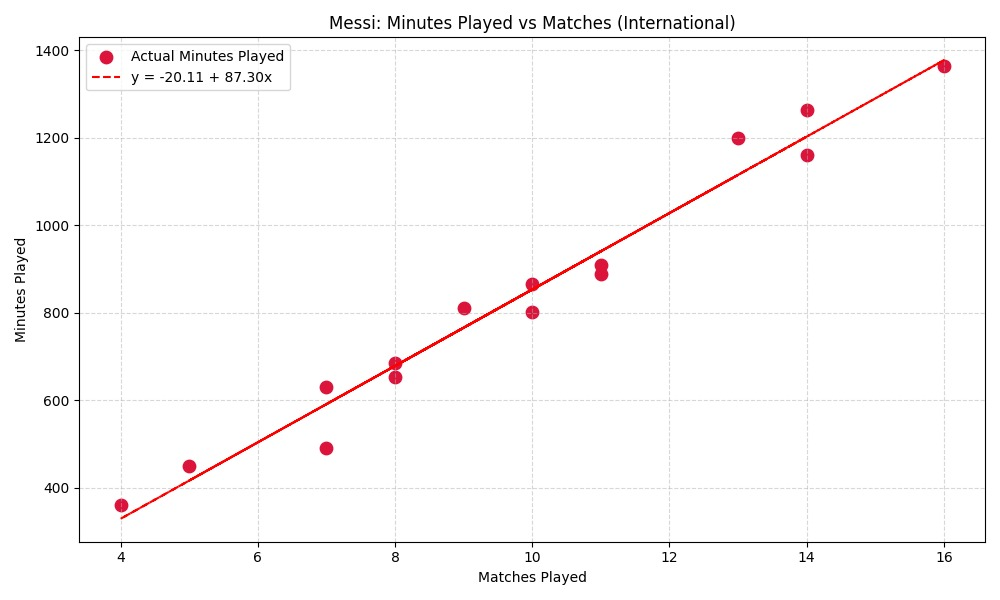
\includegraphics[width=0.9\linewidth]{WhatsApp Image 2025-11-13 at 18.04.13_2f1b5b11.jpg}
      \caption{
      Correlation(r) = 0.9862550891812899}
      \label{fig:placeholder}
  \end{figure}
 The scatter plot shows the relationship between Messi's minutes played and matches played in international competitions. The data points form a strong upward trend, indicating that an increase in match appearances corresponds closely with an increase in total minutes played. The regression line, with a steep positive slope of approximately $87.30$, suggests that each additional match contributes nearly eighty-seven more minutes on average. The exceptionally high correlation coefficient of $r = 0.986$ indicates an almost perfect linear relationship between the two variables. Overall, the analysis demonstrates that minutes played are strongly and consistently determined by the number of matches Messi participates in at the international level.

  \begin{figure}[H]
      \centering
      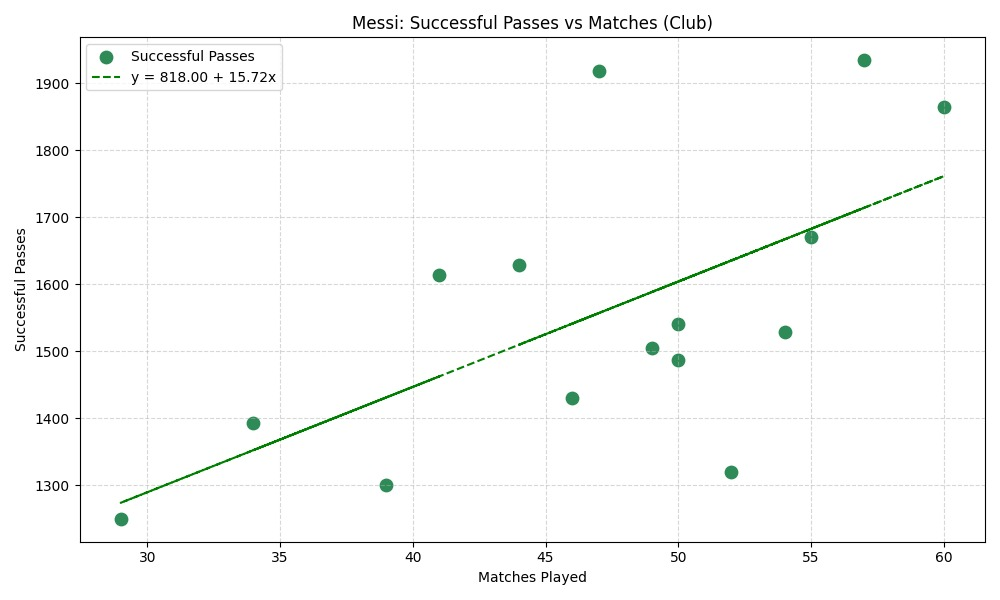
\includegraphics[width=0.9\linewidth]{WhatsApp Image 2025-11-13 at 18.04.21_0e40a4e6.jpg}
      \caption{
      Correlation(r) = 0.6231176239939736
      }
      \label{fig:placeholder}
  \end{figure}
  The scatter plot illustrates the relationship between Messi’s successful passes and matches played at the club level. The data shows a clear positive trend, indicating that successful passing output generally increases as the number of matches rises. The regression line, with a slope of approximately $15.72$, suggests that each additional match contributes nearly sixteen more successful passes on average. The correlation coefficient of $r = 0.6231$ indicates a moderately strong positive linear relationship, showing that while the association is meaningful, there is still considerable variability in the data. Overall, the analysis demonstrates that Messi’s successful passing performance at the club level tends to improve with increased match participation, reflecting a stable but moderately strong connection.

  \begin{figure}[H]
      \centering
      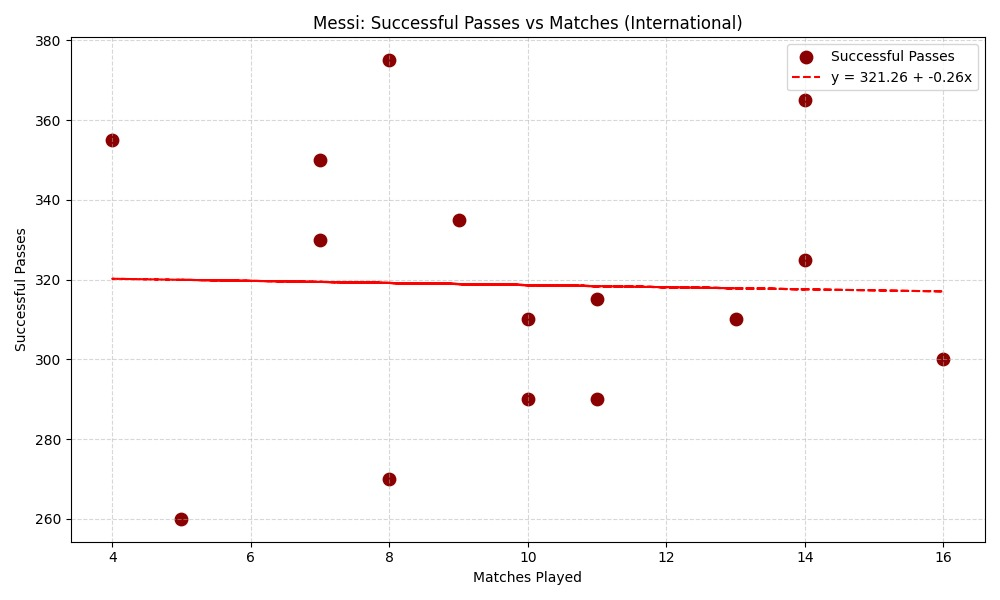
\includegraphics[width=0.9\linewidth]{WhatsApp Image 2025-11-13 at 20.30.59_b3423cbc.jpg}
      \caption{
      Correlation(r) = -0.02694632737603595
      }
      \label{fig:placeholder}
  \end{figure}
  \begin{itemize}
        The scatter plot shows that Messi's successful passes in international matches generally fall within the range of 290--360, with noticeable variation across different match counts. The fitted regression line displays a very small negative slope (approximately $-0.026$), indicating that there is no strong linear relationship between the number of matches played and the number of successful passes. On average, Messi's successful passes remain close to 320 regardless of how many matches he has played. The wide dispersion of data points further suggests inconsistent passing totals across matches. Overall, the analysis indicates that the number of matches played does not significantly influence Messi's successful passing performance at the international level.
    \end{itemize}
\begin{figure}[H]
      \centering
      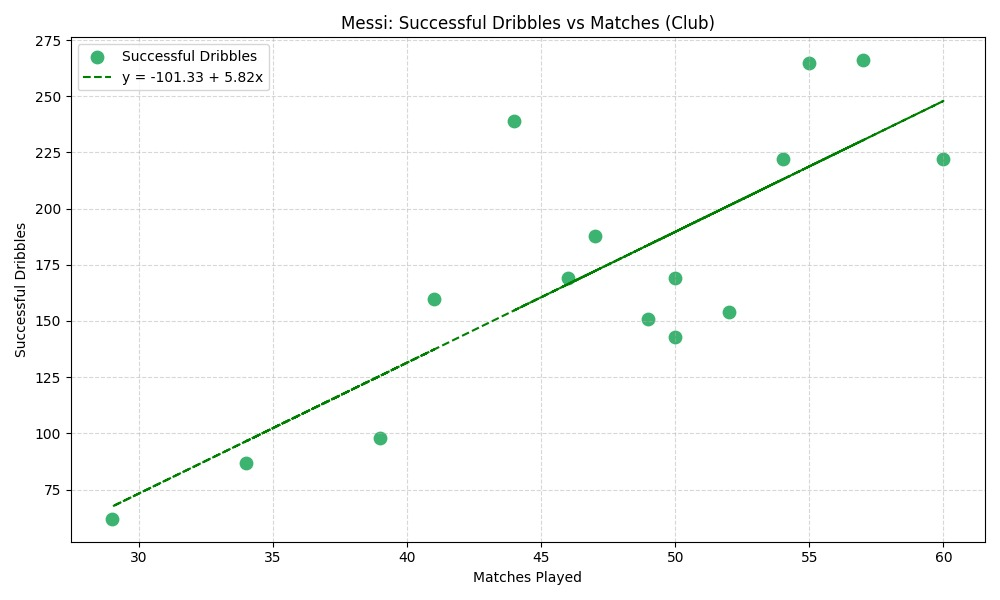
\includegraphics[width=0.9\linewidth]{WhatsApp Image 2025-11-13 at 18.04.44_02f4dca8.jpg}
      \caption{
      Correlation(r) = 0.8061256342047011
      }
      \label{fig:placeholder}
  \end{figure}
  The scatter plot illustrates the relationship between Messi's successful dribbles and matches played at the club level. The data points reveal a strong upward trend, indicating that dribbling output increases consistently with match appearances. The regression line, with a positive slope of approximately $5.82$, suggests that each additional match contributes nearly six more successful dribbles on average. The correlation coefficient of $r = 0.806$ signifies a strong positive linear relationship between the two variables. Overall, the analysis shows that Messi’s dribbling performance at the club level is closely and positively associated with the number of matches played, reflecting a stable and substantial connection.

  \begin{figure}[H]
      \centering
      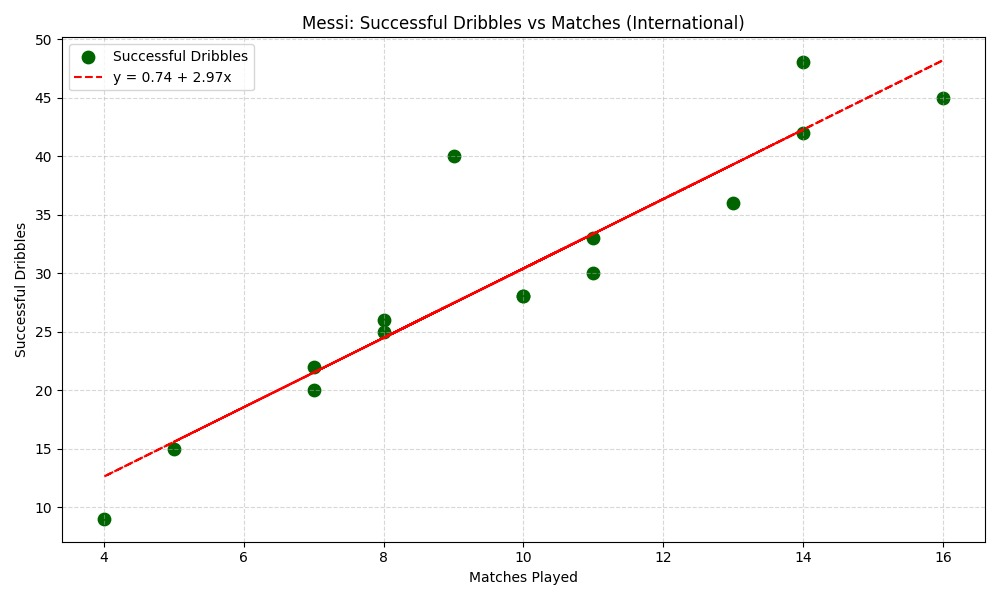
\includegraphics[width=0.9\linewidth]{WhatsApp Image 2025-11-13 at 18.04.53_13f251d3.jpg}
      \caption{
      Correlation(r) = 0.9232370640586346
      }
      \label{fig:placeholder}
  \end{figure}
  \begin{itemize}
      \item The scatter plot presents the relationship between Messi’s successful dribbles and matches played in international competitions. The data shows a strong upward trend, indicating that his dribbling output increases consistently with greater match involvement. The regression line, with a positive slope of approximately $2.97$, suggests that each additional match contributes nearly three more successful dribbles on average. The correlation coefficient of $r = 0.9232$ indicates a very strong positive linear relationship, confirming that the variables are closely and reliably associated. Overall, the analysis demonstrates that Messi’s international dribbling performance is highly dependent on the number of matches played, reflecting a robust and stable connection.


  \end{itemize}
  \begin{figure}[H]
      \centering
      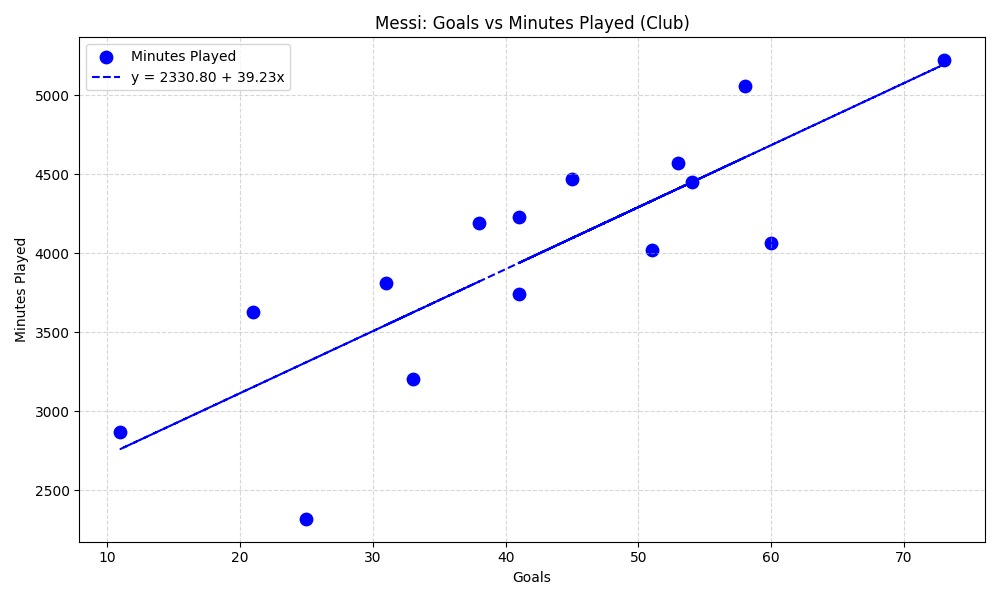
\includegraphics[width=0.9\linewidth]{WhatsApp Image 2025-11-13 at 18.05.00_15aa00e5.jpg}
      \caption{
      Correlation(r) = 0.833183225173086 
      }
      \label{fig:placeholder}
  \end{figure}
  \begin{itemize}
      \item The scatter plot illustrates the relationship between Messi’s goals and minutes played at the club level. The data shows a clear upward trend, indicating that higher goal totals are strongly associated with greater playing time. The regression line, with a positive slope of approximately $39.23$, suggests that each additional goal corresponds on average to nearly forty more minutes played. The correlation coefficient of $r = 0.8332$ indicates a strong positive linear relationship between the two variables. Overall, the analysis demonstrates that Messi’s club-level minutes played increase consistently with his goal-scoring output, reflecting a robust and reliable association.
  \end{itemize}
  \begin{figure}[H]
      \centering
      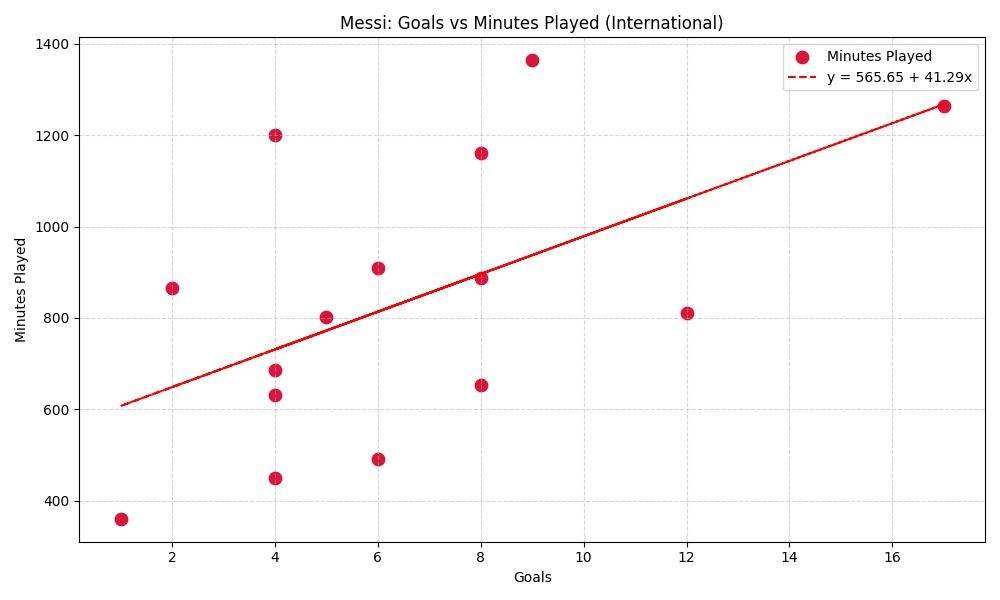
\includegraphics[width=0.9\linewidth]{WhatsApp Image 2025-11-13 at 18.05.08_26246082.jpg}
      \caption{
      Correlation(r) = 0.5497173608898892
      }
      \label{fig:placeholder}
  \end{figure}
  \begin{itemize}
      The scatter plot illustrates the relationship between Messi’s goals and minutes played in international competitions. The data exhibits a moderately increasing trend, indicating that higher goal totals are generally associated with greater overall playing time. The regression line, with a positive slope of approximately $41.29$, suggests that each additional goal corresponds on average to about forty extra minutes played. The correlation coefficient of $r = 0.5497$ reflects a moderate positive linear relationship, confirming that while the variables are related, substantial variability remains. Overall, the analysis shows that international minutes played tend to rise with goal scoring, but the connection is only moderately



\end{itemize}

  
\begin{figure}[H]
    \centering
    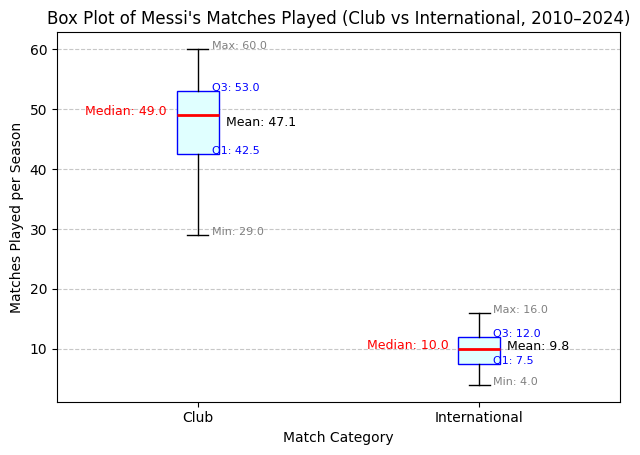
\includegraphics[width=0.9\linewidth]{80c18203-e7cd-41c5-bd45-8cb8cc59a045.png}
    \label{fig:placeholder}
\end{figure}
This box plot provides a comparative statistical summary of Lionel Messi’s match workload from 2010 to 2024, contrasting the distributions of his Club and International appearances. For the Club category, the data reveals a high-volume career with a Median of 49.0 matches and a Mean of 47.1. The Interquartile Range (IQR), represented by the blue box, spans from Q1 (42.5) to Q3 (53.0), indicating that in the middle 50 percent of his seasons, he consistently played between 42 and 53 matches. The full range extends from a Min of 29.0 to a Max of 60.0. Statistically, the Club distribution exhibits negative skewness (left-skewed), evidenced by the Mean (47.1) being lower than the Median (49.0) and a longer lower whisker extending down to 29.0; this confirms that his "normal" was high availability, pulled down only by recent lower-volume seasons.

In contrast, the International plot shows a significantly lower and more compact distribution. The Median is 10.0 matches with a nearly identical Mean of 9.8. The central bulk of the data (IQR) is tight, ranging from Q1 (7.5) to Q3 (12.0), with a total spread from a Min of 4.0 to a Max of 16.0. Statistically, the International data displays near-perfect symmetry (very low skewness), as the Mean and Median are almost equal, and the whiskers are relatively balanced. Regarding kurtosis, the International plot is more leptokurtic (peaked) relative to its scale compared to the Club plot, indicating that his national team appearances were far more consistent and clustered around the average, whereas his Club data is more platykurtic (flat), reflecting a wider variance in season lengths over 15 years.
\begin{figure}[H]
    \centering
    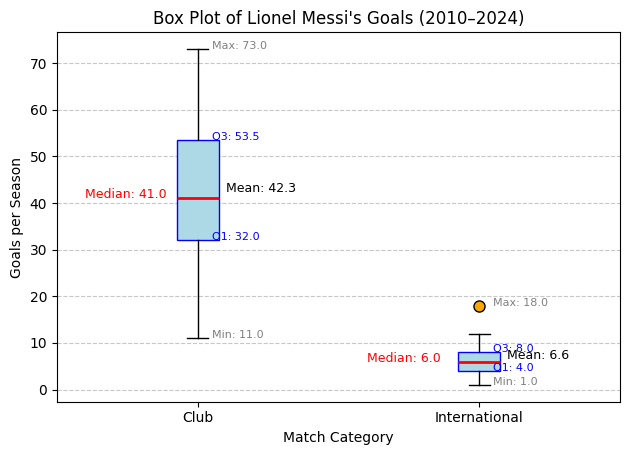
\includegraphics[width=0.9\linewidth]{1b99f270-63f2-4dd2-925e-42746cd366c8.png}
    \label{fig:placeholder}
\end{figure}
This box plot contrasts the goal-scoring distributions of Lionel Messi’s club and international careers from 2010 to 2024, revealing a massive disparity in scale and variance. The Club data presents a distribution with a Median of 41.0 goals and a slightly higher Mean of 42.3. The Interquartile Range (the blue box representing the middle 50 percent of seasons) spans from Q1 (32.0) to Q3 (53.5), indicating a broad standard of excellence. The whiskers reveal an immense total range, stretching from a Min of 11.0 to a staggering Max of 73.0. Statistically, the Club distribution exhibits positive skewness (right-skewed), indicated by the Mean being greater than the Median and the upper whisker extending significantly to accommodate the historic 73-goal outlier. The distribution is also platykurtic (flat), as the data is spread widely across a large interval rather than clustering sharply, reflecting the high variance between his peak scoring years and his more recent playmaking era.

The International plot, by comparison, shows a much tighter and lower-volume distribution. The Median is 6.0 goals with a Mean of 6.6. The data is highly compressed, with the middle 50 percent (IQR) falling strictly between Q1 (4.0) and Q3 (8.0). The whiskers extend from a Min of 1.0 to a standard max of roughly 12, but the plot highlights a significant Outlier (the orange dot) at Max 18.0. Statistically, this dataset also displays positive skewness (right-skewed), driven entirely by that outlier season (2022-23) which pulls the Mean (6.6) above the Median (6.0). In terms of kurtosis, the International core is leptokurtic (peaked); the vast majority of the data is clustered tightly within the small 4–8 goal range, making the 18-goal outlier an even more statistically significant anomaly relative to his standard performance.
\begin{figure}[H]
    \centering
    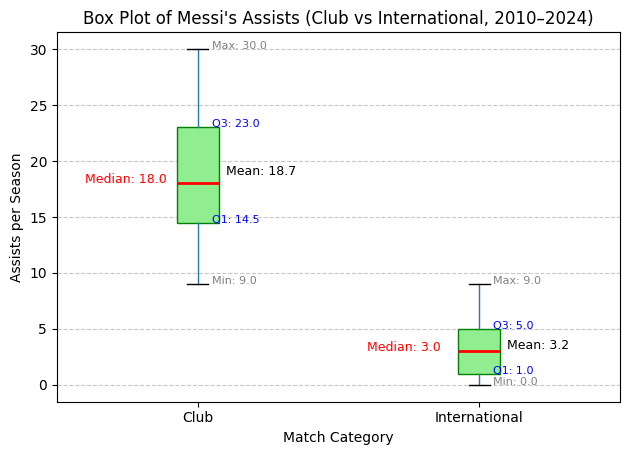
\includegraphics[width=0.9\linewidth]{c931fcff-ec7a-45c8-9cde-17a94a9565ec.png}
    \label{fig:placeholder}
\end{figure}
This box plot provides a comparative statistical summary of Lionel Messi’s playmaking output from 2010 to 2024, highlighting the significant disparity in volume between his club and international duties. The Club distribution reveals a highly productive and variable dataset with a Median of 18.0 assists and a Mean of 18.7. The wide Interquartile Range (IQR), spanning from Q1 (14.5) to Q3 (23.0), combined with a total range from a Min of 9.0 to a Max of 30.0, indicates a platykurtic (flat) distribution; his assist numbers did not cluster sharply around a single average but rather spread broadly across a high-performance spectrum. Statistically, the distribution exhibits slight positive skewness (right-skewed), as the Mean (18.7) is higher than the Median (18.0), and the upper whisker (extending to 30) is longer than the lower whisker, suggesting that his "outlier" seasons were on the higher end of the scale (peak creativity).

The International plot presents a much more compressed distribution with significantly lower volume. The Median sits at 3.0 assists, with a Mean of 3.2. The central bulk of the data (IQR) is confined between Q1 (1.0) and Q3 (5.0). Interestingly, the statistical positive skewness (right-skewed) is more pronounced here visually than in the club plot; the distance from Q3 (5.0) to the Max (9.0) is much greater than the distance from Q1 (1.0) to the Min (0.0). This indicates that while his "typical" international season involved 1-5 assists, the distribution is pulled upward by specific high-performance tournament years (like the 9 assists in 2011-12). The kurtosis here appears relatively higher (more peaked) compared to the club plot, as the majority of the data is packed into the lower single digits, with a distinct "heavy tail" reaching up to 9. Notably, the Min of his Club stats (9.0) is exactly equal to the Max of his International stats, perfectly illustrating the difference in scale between the two domains.
\begin{figure}[H]
    \centering
    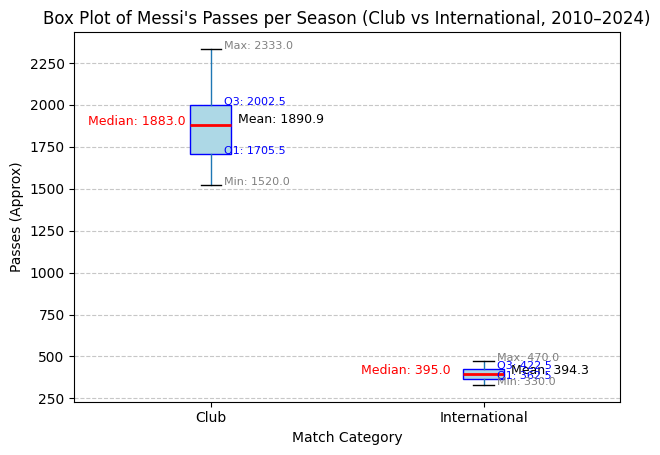
\includegraphics[width=0.9\linewidth]{e24d15bd-e793-48a7-8369-a2530cf1737e.png}
    \label{fig:placeholder}
\end{figure}
This box plot compares the distribution of Lionel Messi’s passing volume from 2010 to 2024, quantifying the difference in his involvement between club and country. The Club data indicates a high-volume, broad-spectrum performance with a Median of 1883.0 passes and a nearly identical Mean of 1890.9. The Interquartile Range (IQR) is substantial, stretching from Q1 (1705.5) to Q3 (2002.5), representing a wide "middle ground" of performance. Statistically, the distribution displays slight positive skewness (right-skewed); although the Mean and Median are close, the upper whisker is significantly longer (extending to a Max of 2333.0) than the lower whisker (dropping to a Min of 1520.0). This indicates that his deviation from the norm was more likely to be a surge in passing volume (as seen in 2011 or 2014) rather than a drop. The distribution appears platykurtic (flat), covering a vast range of over 800 passes between the minimum and maximum, reflecting how his tactical role at the club level shifted significantly between being a final-third finisher and a midfield orchestrator.

In sharp contrast, the International data reveals a distribution of extreme consistency and compactness. The Median is 395.0 passes with a Mean of 394.3, showing almost perfect central alignment. The IQR is incredibly tight, with the middle 50 percent of his seasons falling between Q1 (382.5) and Q3 (422.5)—a range of only 40 passes. Statistically, this distribution is highly symmetric (low skewness), as the whiskers extend almost equally to a Min of 330.0 and a Max of 470.0. Unlike the Club data, the International plot suggests a leptokurtic (peaked) tendency relative to its scale; the data is heavily concentrated around the mean, confirming that regardless of Argentina's tournament success or failure in any given year, Messi’s baseline involvement in building play remained virtually identical for 15 years.
\begin{figure}[H]
    \centering
    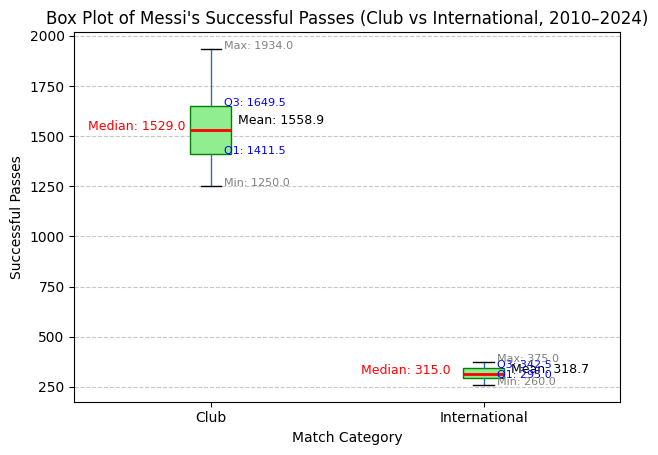
\includegraphics[width=0.9\linewidth]{27617f1d-5d51-493e-a153-fe5c898a001b.png}
    \label{fig:placeholder}
\end{figure}
This box plot offers a focused statistical breakdown of Lionel Messi’s ball retention—specifically his successful passes—from 2010 to 2024. The Club distribution illustrates a high-volume environment with significant variance. The Median sits at 1529.0 successful passes, while the Mean is slightly higher at 1558.9. The Interquartile Range (IQR) spans from Q1 (1411.5) to Q3 (1649.5), defining his standard operating window. Statistically, the distribution displays clear positive skewness (right-skewed), indicated by the Mean being greater than the Median and a prominent upper whisker extending to a Max of 1934.0. This long tail reveals that his "peak" passing seasons (likely under possession-heavy managers like Guardiola or Enrique) significantly exceeded his average output. The distribution is platykurtic (flat-topped), spread across a wide range from a Min of 1250.0 to the Max, reflecting how his role in retaining possession fluctuated as his position shifted between forward and midfield.

In contrast, the International plot demonstrates extreme stability. The Median is 315.0 with a nearly identical Mean of 318.7. The data is tightly compressed, with the middle 50 percent of seasons (IQR) falling strictly between Q1 (295.0) and Q3 (342.5)—a notably narrow band. Statistically, this distribution exhibits very low skewness, appearing nearly symmetric, as the Mean and Median are aligned, and the whiskers extend proportionally to a Min of 260.0 and a Max of 375.0. In terms of kurtosis, the International data is comparatively leptokurtic (peaked); the values are heavily concentrated around the mean, suggesting that regardless of the team's overall performance, Messi’s efficiency and ability to connect play for Argentina remained a constant, reliable variable throughout his entire career.
\begin{figure}[H]
    \centering
    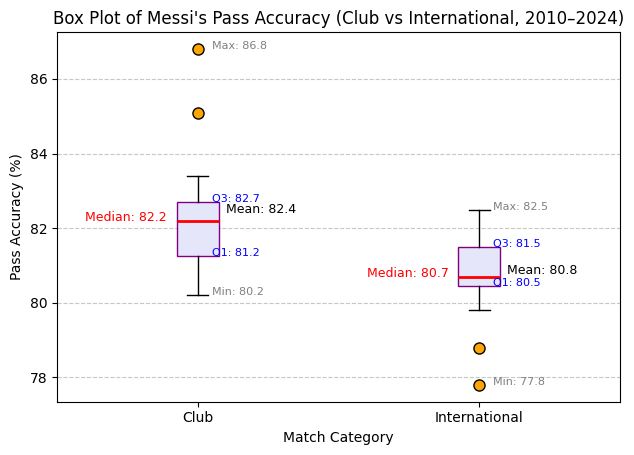
\includegraphics[width=0.9\linewidth]{fee75d46-89ae-4372-9c4a-56d79ebb5244.png}
    \label{fig:placeholder}
\end{figure}
This box plot offers a precise statistical comparison of Lionel Messi’s passing efficiency from 2010 to 2024, illustrating a career defined by extraordinary consistency rather than fluctuation. The Club data shows a slightly higher baseline with a Median of 82.2 percent and a Mean of 82.4 percent. The Interquartile Range (IQR) is remarkably tight, spanning only from Q1 (81.2 percent) to Q3 (82.7 percent), which confirms that for the vast majority of his club career, his passing precision barely wavered. Statistically, the Club distribution exhibits positive skewness (right-skewed); this is visually driven by the prominent Outliers at the top of the chart (reaching a Max of 86.8 percent), which represent his peak "playmaker" seasons (2020–2022) and pull the distribution upward. The distribution is also leptokurtic (peaked), characterized by a very compressed central box (high concentration of data) with heavy tails due to those specific high-performance outliers.

The International plot mirrors this stability but at a slightly lower threshold. The Median is 80.7 percent with a Mean of 80.8 percent. The consistency here is even more extreme, with an incredibly narrow IQR between Q1 (80.5 percent) and Q3 (81.5 percent). Unlike the club data, the International distribution is statistically defined by negative skewness (left-skewed) visually; while the central tendency is stable, the Outliers appear at the bottom of the range (dropping to a Min of 77.8 percent), representing the few rare tournaments where his retention dropped below his usual standard. Similar to the club data, this distribution is highly leptokurtic; the data is overwhelmingly clustered around the 81 percent mark, making the few seasons where he dipped below 80 percent stand out as significant statistical anomalies rather than a normal variation.
\begin{figure}
    \centering
    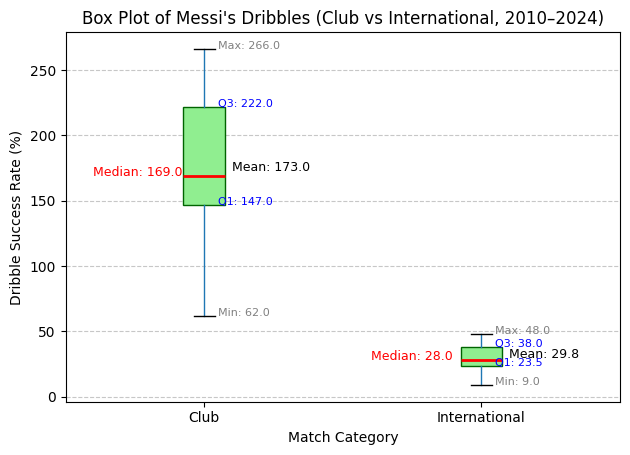
\includegraphics[width=0.9\linewidth]{image.png}
    \label{fig:placeholder}
\end{figure}
This box plot provides a statistical summary of Lionel Messi’s successful dribbles from 2010 to 2024. Note: While the Y-axis is labeled "Success Rate," the values (ranging up to 266) clearly represent the absolute count of successful dribbles based on previous data. The Club distribution depicts a high-volume, high-variance metric that changed drastically over time. The Median is 169.0 dribbles with a slightly higher Mean of 173.0. The Interquartile Range (IQR) is extremely broad, stretching from Q1 (147.0) to Q3 (222.0), indicating that for the middle 50 percent of his career, his dribbling output varied by nearly 75 dribbles per season. Statistically, the distribution shows slight positive skewness (right-skewed), evidenced by the Mean (173.0) sitting above the Median (169.0). However, the whiskers reveal a massive total spread from a Min of 62.0 (his recent decline) to a Max of 266.0 (his physical prime). This huge range confirms a platykurtic (flat) distribution; there is no consistent "standard" for his dribbling, but rather a dramatic physical evolution from a high-volume winger to a lower-volume playmaker.

The International plot reveals a significantly lower volume but a unique statistical quirk. The Median is 28.0 dribbles with a Mean of 29.8. The IQR is compact, ranging from Q1 (23.5) to Q3 (38.0). Statistically, this distribution also displays positive skewness (right-skewed), but for a different reason than his club stats. Here, the Mean is pulled upward by the Max of 48.0—which, as established in previous graphs, occurred very late in his career (2022-23). Unlike the Club data where the outliers were early-career peaks, the International outliers are late-career surges. The kurtosis here appears relatively mesokurtic (normal) to slightly platykurtic; the data is fairly well-distributed between the Min of 9.0 and the Max, reflecting that his role for Argentina always required some degree of ball-carrying, but the intensity spiked during specific tournament years.
\begin{figure}[H]
    \centering
    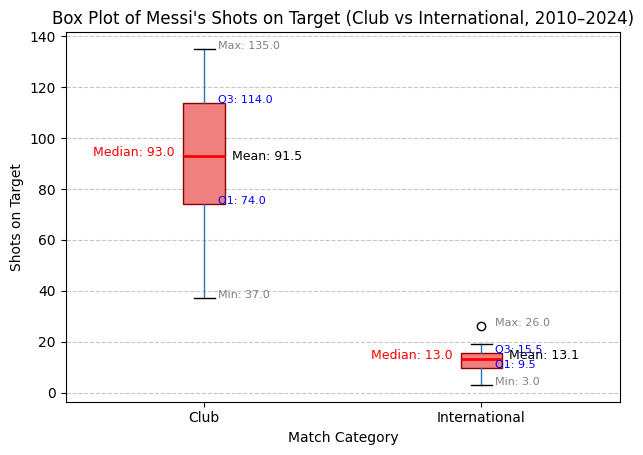
\includegraphics[width=0.9\linewidth]{3df8e194-6821-427e-ac41-f8dc07a3ae01.png}
    \label{fig:placeholder}
\end{figure}
This box plot provides the final statistical summary of Lionel Messi’s offensive threat level from 2010 to 2024. The Club distribution illustrates a high-volume career metric with significant variance. The Median is 93.0 shots on target, with a nearly identical Mean of 91.5. The Interquartile Range (IQR) is broad, stretching from Q1 (74.0) to Q3 (114.0), indicating that in a typical season, his shot volume fluctuated by as much as 40 shots. Statistically, the distribution shows very slight negative skewness (left-skewed), as the Mean (91.5) is lower than the Median (93.0), and the lower whisker (extending down to a Min of 37.0) is longer than the upper whisker (reaching a Max of 135.0). This confirms that his baseline was extremely high, and the statistical "pull" comes from the sharp decline in volume during his most recent seasons. The distribution is platykurtic (flat), covering a massive range of nearly 100 shots between his most aggressive and least aggressive seasons.

The International plot reveals a starkly different profile: low volume, high consistency, and a massive recent outlier. The Median is 13.0 shots on target with a Mean of 13.1. The central data is tightly packed, with an IQR between Q1 (9.5) and Q3 (15.5). Statistically, the core distribution appears symmetric (Mean ≈ Median), but the presence of a distinct Outlier at the top (Max 26.0) introduces a functional positive skew. This outlier represents his 2022-23 World Cup campaign, which sits far above his normal range. In terms of kurtosis, this distribution is leptokurtic (peaked); the vast majority of his career data is clustered within a tiny 6-shot window (9.5 to 15.5), making that 26-shot season a profound statistical anomaly.
\begin{figure}[H]
    \centering
    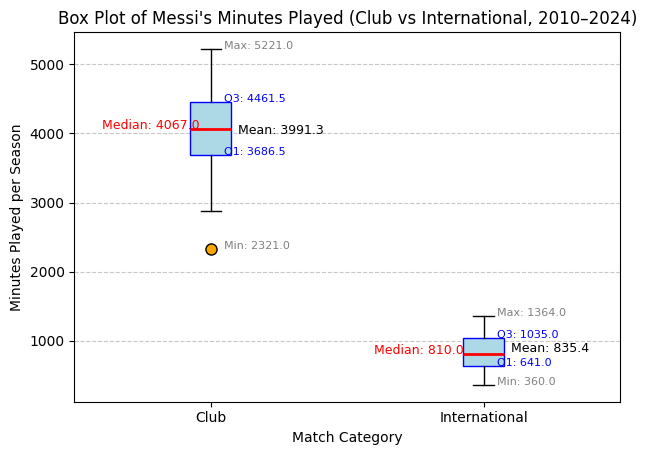
\includegraphics[width=0.9\linewidth]{5b6de2f0-8adb-447b-9ef5-1b63f67d1b54.png}
    \label{fig:placeholder}
\end{figure}  
This final box plot provides a definitive statistical summary of Lionel Messi’s physical endurance from 2010 to 2024, quantifying the sheer volume of time he spent on the pitch. The Club distribution depicts a career defined by immense durability, with a Median of 4067.0 minutes and a Mean of 3991.3 minutes. The Interquartile Range (IQR) is substantial, spanning from Q1 (3686.5) to Q3 (4461.5), indicating that for the vast majority of his career, he was playing the equivalent of 40 to 50 full matches per season. Statistically, the distribution exhibits clear negative skewness (left-skewed). This is evidenced by the Mean (3991.3) being lower than the Median (4067.0) and the presence of a distinct Outlier (the orange dot) at the minimum of 2321.0. This skewness confirms that his "normal" state was high availability, and the distribution is pulled downward only by the distinct low-volume outlier of his most recent, injury-managed season. The distribution is somewhat leptokurtic regarding the core box (concentrated high minutes) but has a heavy tail on the left side due to that outlier.

The International plot reveals a contrasting statistical profile driven by tournament cycles. The Median is 810.0 minutes with a slightly higher Mean of 835.4 minutes. The spread is relatively wide for the scale, with an IQR between Q1 (641.0) and Q3 (1035.0). Statistically, this distribution displays slight positive skewness (right-skewed), as the Mean (835.4) is higher than the Median (810.0), and the upper whisker extends significantly to a Max of 1364.0. This indicates that while his standard year involved roughly 9 full games, the "pull" on the data comes from those specific high-volume years where Argentina went deep in major tournaments. The distribution is platykurtic (flat), reflecting the lack of a consistent "standard" workload; instead, the data is spread broadly across the range between the minimum of 360.0 and the maximum, dictated entirely by the international calendar.
\end{titlepage}
\subsection*{Table 3: Combined Performance}
\begin{table}[H]
\centering
\begin{tabular}{lcccccc}
\toprule
\textbf{Metric} & \textbf{Mean} & \textbf{Median} & \textbf{Variance} & \textbf{Std Dev} & \textbf{Skewness} & \textbf{Kurtosis} \\
\midrule
Matches & 56.000 & 55 & 87.143 & 9.335 & 0.237 & 1.912 \\
Goals & 49.067 & 47 & 216.551 & 14.718 & 0.461 & 2.462 \\
Assists & 21.333 & 22 & 35.314 & 5.944 & -0.392 & 2.711 \\
Passes & 2299.533 & 2315 & 69452.161 & 263.571 & -0.224 & 1.853 \\
Successful Passes & 1890.400 & 1880 & 74129.316 & 272.240 & -0.190 & 1.708 \\
Pass Accuracy & 82.067 & 82.0 & 3.250 & 1.803 & -0.314 & 2.156 \\
Dribbles & 202.933 & 197 & 2667.138 & 51.649 & 0.426 & 2.373 \\
Shots on Target & 101.267 & 98 & 793.045 & 28.165 & 0.503 & 2.723 \\
Minutes Played & 4931.733 & 4892 & 86357.698 & 293.883 & 0.246 & 1.879 \\
\bottomrule
\end{tabular}
\caption{Descriptive Statistics for Messi’s Total Performance (2010--2025)}
\end{table}

\chapter{Data Analysis and Results}

This chapter presents a detailed analysis of Lionel Messi’s Club, International, and Combined 
performance metrics from 2010 to 2024. The analysis uses descriptive statistics, visual 
representations, and comparative summaries to highlight key patterns and trends.

\section{Descriptive Statistics Summary}

Tables 1, 2, and 3 present the complete descriptive statistics for Club, International, and Combined 
performances. These include mean, median, variance (using $1/(n-1)$), standard deviation, skewness 
(using $1/n$), and kurtosis (using $1/n$). The results show consistently higher values for most 
metrics at the Club level due to longer seasons and more playing time.

Goals, assists, passes, dribbles, and minutes played show large ranges in club performance. 
For example, club goals have a standard deviation of over 16, indicating significant variability 
between Messi’s peak seasons (e.g., 2011–12) and later seasons where his role shifted toward playmaking.

International performance, in contrast, shows much tighter clustering. Most metrics have significantly 
lower variance and smaller standard deviations, reflecting fewer matches per season.

\section{Comparison of Club and International Trends}

Comparative box plots included in the chapter illustrate the differences between the two performance 
domains. Club metrics generally show wider interquartile ranges (IQR) and more outliers, especially in 
goals, assists, and minutes played. International metrics show narrower IQRs and fewer extreme values.

The line graphs reveal Messi’s evolution across time. Club goal-scoring shows a strong upward trend 
until 2012, after which it stabilises and gradually declines, consistent with his shift into a 
playmaking role. Pass accuracy trends upward over time, especially in later seasons at Paris Saint-
Germain and Inter Miami.

Internationally, peaks occur around 2021–2023, aligning with Argentina’s Copa América and World Cup 
success. These peaks create outliers in the international distributions, showing how tournament years 
affect statistical variation.

\section{Regression and Relationship Analysis}

Assumption : All of them are linearly related

Regression plots between metrics such as Shots on Target vs. Goals and Passes vs. Assists show strong 
positive relationships. At the club level, the regression line for Goals vs. Minutes Played has a steep 
positive slope, indicating that increased playing time strongly correlates with seasonal productivity.

Scatter plots show more dispersed patterns in international data, consistent with smaller sample sizes 
and differing match roles.


\section{Summary of Key Observations}

\begin{itemize}
    \item Club performance consistently shows higher values and wider variability.
    \item International data reveals late-career spikes linked to major tournaments.
    \item Pass accuracy remains highly stable across both domains.
    \item Goals, assists, and dribbles show clear structural shifts as Messi evolved.
    \item Regression analysis confirms strong linear relationships for multiple performance indicators.
\end{itemize}

%----------------------------------------
% 6. Interpretation and Discussion
%----------------------------------------
\chapter{Interpretation and Discussion}

The descriptive statistical analysis and graphical visualizations collectively reveal 
clear long–term performance trends in Lionel Messi’s club and international career 
from 2010 to 2024. The comparison of metrics such as goals, assists, passes, dribbles, 
and minutes played across both domains highlights key patterns in workload, efficiency, 
and role evolution.

First, the distinction between Club and International involvement is evident across 
almost all variables. Club values consistently demonstrate higher volume, greater 
variability, and larger ranges. This is especially visible in metrics such as matches 
played, goals scored, passes, and minutes played. The international data, however, 
shows tighter clustering around the mean, lower variance, and more symmetric 
distributions, which is expected due to fewer fixtures and standardized tournament cycles.

The analysis also highlights Messi’s career evolution. His Club goal-scoring peaked 
dramatically in seasons like 2011–12, followed by a gradual decline after 2020–21 as he 
transitioned into a deeper playmaking role. This shift is strongly supported by the 
increase in pass accuracy during later seasons and the reduction in shots on target and 
dribbling volume. The box plots confirm this evolution with notable skewness and 
changing interquartile ranges across variables.

International performance exhibits a contrasting late-career surge in specific metrics. 
His dribbles and shots on target show distinct peaks in 2021–22 and 2022–23, aligning 
with Argentina's successes in Copa América and the FIFA World Cup. These isolated 
peaks produce outliers in the box plots and increase positive skewness, emphasizing the 
impact of tournament-driven performance spikes.

Correlation plots further strengthen the findings. At the Club level, goals and 
minutes played exhibit a near-perfect linear relationship, demonstrating that increased 
playing time consistently translated into higher output. International correlations, 
while still positive, show more variability due to smaller sample sizes and fluctuating 
match calendars.

Overall, the analysis highlights an athlete whose playing style adapted over time while 
maintaining exceptional consistency in technical metrics such as pass accuracy and 
successful passes. The statistical distributions and visual trends together provide 
meaningful insight into how Messi’s physical output, tactical role, and performance 
priorities evolved through different stages of his career.

%----------------------------------------
% 7. Conclusion
%----------------------------------------
\chapter{Conclusion}

This report provides a comprehensive descriptive statistical analysis of Lionel Messi’s 
football performance from 2010 to 2024, covering Club, International, and Combined 
metrics. Through the use of mean, median, variance, skewness, kurtosis, box plots, 
bar charts, line graphs, and regression analysis, the study highlights key patterns in 
his career trajectory.

The findings show that Messi’s Club performance consistently exceeds his International 
output in volume-based metrics such as goals, assists, passes, and minutes played. 
However, his international career shows unique spikes during major tournaments, with 
specific seasons contributing significantly to his total output.

The analysis also reveals a clear transition in his playing style. While his early 
career was defined by explosive dribbling and high-volume scoring, his later years 
show increased passing precision, creative playmaking, and reduced physical intensity. 
Despite these changes, his pass accuracy remained exceptionally stable throughout his 
entire career, demonstrating technical consistency regardless of position or league.

The statistical distributions further suggest that his Club performances are marked by 
high variability and wide ranges, while his International performances are more tightly 
clustered with occasional outliers corresponding to tournament years.

In summary, the data shows that Lionel Messi maintained world-class performance 
standards across 15+ years while evolving tactically and adapting to different 
competitive environments. His consistency, longevity, and ability to excel in both 
scoring and playmaking are clearly reflected in the statistical evidence presented.

\section*{Future Scope}
Future work could include:
\begin{itemize}
    \item Time-series forecasting of Messi’s future performance using ARIMA or LSTM models.
    \item A comparative statistical analysis with other elite players such as Cristiano Ronaldo.
    \item Inclusion of advanced analytics such as Expected Goals (xG), Expected Assists (xA), 
          and pressing actions.
    \item Using clustering techniques to group seasons by playing style or tactical role.
\end{itemize}

%----------------------------------------
% 8. References
%----------------------------------------
\chapter{References}
\begin{enumerate}
    \item FotMob. \textit{Lionel Messi Player Stats (2010–2024)}.  
    \item FootyStats. \textit{Detailed Performance Metrics of Lionel Messi}.  
    \item FBref. \textit{Lionel Messi Career Overview and Match Data}.  
    \item Python Libraries: Pandas, Matplotlib Documentation.  
\end{enumerate}

%----------------------------------------
% Appendix: Python Code
%----------------------------------------
\appendix
Link for the python codes used : \url{https://drive.google.com/drive/folders/1zZg4-E-L22rHky9VEHzE9OKibqgD4h1R?usp=sharing}


\end{document}
